\documentclass[12pt,a4paper]{cibb}
\usepackage{pgfplotstable} % More robust CSV table handling
\usepackage{float} %Used for [H] in figures to place exactly under where text is in latex



% Fallback definition for missing \@ordinalM
\makeatletter
\providecommand{\@ordinalM}[2]{#1}
\makeatother

\usepackage{subfigure,graphicx}
\usepackage{amsmath,amsfonts,latexsym,amssymb,euscript,xr}
\usepackage{booktabs}
\usepackage[nodayofweek]{datetime}
\usepackage{hyperref}
\usepackage{fmtcount}
\usepackage[english]{datenumber}
\usepackage[absolute]{textpos}

\usepackage[table]{xcolor}
\usepackage{color,colortbl,tabularx}
\usepackage[english]{babel}
\usepackage[protrusion=true,expansion=true]{microtype}
\usepackage{amsmath,amsfonts,amsthm}
\usepackage{pifont}
\usepackage{array}
\usepackage{longtable}
\usepackage{multirow}
\usepackage{url}

\usepackage{graphicx} % Used for reading png(s)
\usepackage{csvsimple} % For reading in csv tables
\usepackage[strings]{underscore} % Helps CSV text render underscores safely

\def\red{\color{red}}
\def\black{\color{black}}
\def\blue{\color{blue}}
\def\magenta{\color{magenta}}

\definecolor{LightBlue}{rgb}{0.88,0.9,0.9}

\newcommand\blfootnote[1]{%
  \begingroup
  \renewcommand\thefootnote{}\footnote{#1}%
  \addtocounter{footnote}{-1}%
  \endgroup
}

\title{\Large $\ $\\ \bf Motion Phase Classification from Biosensor Data}

\author{\blue \large Sneha Basnet$^1$, Nathan Montero$^2$, Sarah Loh$^3$, Aye Nyein Kyaw$^4$, Nurislam Saliev$^5$}
\address{\blue \footnotesize $\ $\\
$^1$ sneha.basnet@sjsu.edu. \\
$^2$ nathan.montero@sjsu.edu. \\
$^3$ sarah.loh@sjsu.edu. \\
$^4$ ayenyein.kyaw@sjsu.edu. \\
$^5$ nurislam.saliev@sjsu.edu \\
 
}

\abstract{\small biosensor data, motion phase classification, wearable sensors, time-series classification. \normalsize
\\[17pt]
{\bf Abstract.} This study presents an end-to-end machine-learning pipeline for the automated classification of motion phases from wearable biosensor data in a track-and-field context. The dataset comprises 1{,}500 timestamped observations from five athletes across six motion-phase categories (Accel, Jump\_Takeoff, Landing, Sprint\_Mid, Start\_Run, and Stop), recorded at 10\,Hz across seven inertial and cardiovascular channels. The pipeline encompasses per-athlete z-score normalisation, sliding-window segmentation, and extraction of time-domain, frequency-domain, and cross-axis correlation features. Seven classical classifiers and a feedforward neural network are evaluated under Stratified 5-Fold Cross-Validation and Leave-One-Subject-Out (LOSO) protocols. Random Forest achieved the best 5-Fold CV accuracy (0.304), MLP the highest test accuracy (0.319), and XGBoost the strongest LOSO performance (0.206), though all models remain near chance ($\approx$0.167) under LOSO. Low accuracy is largely a consequence of label noise from rapidly-transitioning event labels within each segmented window. These findings underscore the importance of subject-independent evaluation and high-fidelity labelling in wearable motion-classification research.

}
\begin{document}

\renewcommand{\thefootnote}{}
\footnotetext{\small{Article version: \datedate $\;$ h\currenttime $\;$ CET}}

\thispagestyle{myheadings}
\pagestyle{myheadings}
\markright{\tt Proceedings of CS 2026}

\section{Introduction}
\label{sec:introduction}

\subsection{Project Overview}
Wearable biosensors are becoming increasingly used in sports science to monitor athlete performance in real time. Devices that simultaneously capture heart rate, three-axis acceleration, and three-axis angular velocity allow coaches and analysts to interpret the biomechanical demands of distinct motion phases without disrupting training sessions. We implemented an end-to-end pipeline for motion phase classification from biosensor data, spanning dataset auditing, signal preprocessing, feature engineering, model training and hyperparameter tuning, and rigorous cross-subject evaluation.

\subsection{Problem Statement}
Manually annotating motion phases from continuous sensor streams is time-consuming and subject to inter-rater variability. Machine learning offers a high-potential alternative, but requires careful signal preprocessing, feature engineering, and validation strategies that account for inter-athlete variability. The core challenge is to train a classifier that generalises to unseen athletes rather than merely memorising within-athlete patterns from a small, single-session dataset with high label noise introduced by sliding-window segmentation.

\subsection{Dataset Summary}
The dataset comprises 1{,}500 timestamped observations from five track-and-field athletes (A001--A005), each contributing 300 samples from a single 30-second recording session at 10\,Hz. Seven sensor channels are available: Heart\_Rate, Acc\_X/Y/Z, and Gyro\_X/Y/Z. Samples are annotated across six balanced motion-phase classes ({\raise.17ex\hbox{$\scriptstyle\sim$}}16.7\% each): Accel, Jump\_Takeoff, Landing, Sprint\_Mid, Start\_Run, and Stop. No demographic metadata is available, which limits generalisation claims across age and sex groups.

\subsection{Report Structure}
Section~\ref{sec:litreview} reviews related literature on wearable motion classification. Section~\ref{sec:DATA} details the methodology across six tasks: dataset exploration, signal exploration, preprocessing, segmentation, feature engineering, and modelling. Section~\ref{sec:results_discussion} presents the consolidated results and discussion, including test-set accuracy, cross-validation comparison, window size analysis, per-class metrics, confusion matrices, and error analysis. Section~\ref{sec:CONCLUSION} concludes with a summary of findings, limitations, and future directions.




\section{Literature Review}
\label{sec:litreview}

\subsection{Validation Methods for Activity Recognition}

A comparative study by Mekruksavanich et al.~\cite{10962074} examined 
the use of $k$-fold and Leave-One-Subject-Out (LOSO) cross-validation 
for sensor-based human activity recognition using deep learning models. 
Their key finding was that high $k$-fold accuracy can be misleading, as 
the model may be tested on activities from the same subjects it was 
trained on. The study used the WISDM dataset, which contains time-series 
data from inertial sensors including accelerometer and gyroscope readings, 
with sliding window segmentation applied prior to modeling. Five deep 
learning architectures were evaluated (CNN, LSTM, BiLSTM, GRU, BiGRU), 
and results supported their thesis: their best model, BiGRU, achieved 
97.91\% accuracy under $k$-fold and 98.02\% under LOSO, demonstrating 
that LOSO can match or exceed $k$-fold in realistic cross-subject 
scenarios. A noted limitation was label ambiguity at motion boundaries, 
which is a challenge shared by our dataset.

\subsection{Effect of Window Size on Activity Recognition}

The choice of window size has been shown to affect the accuracy of 
activity recognition models, particularly when using smartwatch sensor 
data~\cite{10689691}. Mekruksavanich et al. investigated the effect of 
sliding window size on recognition performance across 11 daily activities, 
testing window durations ranging from 5 to 40 seconds using deep learning 
models on smartwatch sensor data. Their results showed that smaller windows 
improved model performance for rapid activity changes, while larger windows 
reduced accuracy in those cases. Although their window size range differs 
substantially from ours, the core finding remains relevant: window sizes 
are both dataset-specific and task-dependent. Classifying sprint phases 
requires fundamentally different temporal resolution than classifying 
everyday activities such as walking.

\subsection{Classifying Motion from Wearable Sensor Data}

Vitali et al.~\cite{Vitali2020} demonstrated that supervised machine 
learning applied to wearable inertial measurement unit (IMU) data can 
accurately classify functional fitness exercises within a continuous 
workout session. Their study used five IMUs placed on the upper and lower 
limbs and trunk of fourteen participants performing four distinct exercise 
types. Time-domain and frequency-domain features were extracted from 
sliding windows and fed into $k$-Nearest Neighbours and Support Vector 
Machine classifiers, achieving high classification accuracy under 
5-fold cross-validation. Their work is directly relevant to our pipeline 
as it validates the use of window-based feature extraction with classical 
ML classifiers for motion phase recognition from IMU data. A key 
limitation noted was that performance was tied to specific body placement 
of sensors, which may not generalize to all wearable configurations.

\subsection{Biosensors and Machine Learning for Athlete Monitoring}

Mekruksavanich and Jitpattanakul~\cite{Mekruksavanich2026} reviewed 
the use of wearable biosensors combined with machine learning for 
data-driven training and coaching support in sports science. Their work 
surveyed physiological signals including heart rate variability, 
accelerometer readings, and gyroscope data, noting that recent AI 
methods have significantly improved real-time signal interpretation and 
motion tracking accuracy. They similarly highlighted 
that multi-sensor fusion, when combining inertial and physiological signals, captures both biomechanical and cardiovascular dimensions of athletic 
activity, which is exactly the structure of our biosensor dataset. 
A limitation of reviewed approaches was that most studies relied on 
controlled laboratory settings, with performance dropping in uncontrolled 
field conditions where sensor noise and label ambiguity are more prevalent.



\subsection{Feature Selection for Sensor Data}

Feature selection plays a critical role in improving classification performance while reducing model complexity. Bennasar et al.~\cite{bennasar2022significant} investigated feature selection methods for human activity recognition using tri-axial accelerometer data. Their results show that selecting a subset of informative features can significantly reduce computational cost while maintaining strong classification accuracy. This supports our use of feature ranking techniques, including mutual information, ANOVA F-statistics, and Random Forest importance, before model training.

A limitation of their work is that it focuses primarily on accelerometer signals, whereas our dataset incorporates multiple sensor modalities, including gyroscope and heart rate. Despite this difference, their findings reinforce the importance of identifying discriminative features prior to model training.

\subsection{Sensor Fusion in Activity Recognition}

Combining multiple sensor modalities has been shown to improve activity recognition performance. Gilmore and Nasseri~\cite{gilmore2024fusion} proposed a human activity recognition system that integrates physiological and inertial signals, including photoplethysmography, electrodermal activity, and accelerometry. Their work demonstrates that combining motion-based and physiological features can enhance classification accuracy by capturing both external movement and internal body state.

This is directly relevant to our project, which integrates heart rate with accelerometer and gyroscope data. While our dataset does not include as many physiological signals as their study, their findings support the design choice of combining multiple sensor types within a single feature-engineering pipeline. A limitation is that their system relies on richer physiological data than what is available in our dataset.


\subsection{Deep Learning and LOSO Validation for Activity Recognition}

Gholamiangonabadi et al.~\cite{9144538} evaluated deep neural networks 
for human activity recognition using wearable sensor data, with a focus 
on Leave-One-Subject-Out (LOSO) cross-validation. Their results show that 
deep models outperform traditional approaches while providing more 
reliable estimates of performance under subject-independent evaluation. 
This highlights the importance of LOSO in avoiding overly optimistic 
results from subject-dependent validation. A limitation is that the study 
uses controlled datasets, which may not fully reflect real-world variability.


\subsection{Hybrid Machine Learning Approaches for Activity Recognition}

Hossain Shuvo et al.~\cite{9425332} proposed a hybrid approach combining 
a 1D convolutional neural network with a support vector machine for human 
activity recognition. The CNN is used for automatic feature extraction 
from time-series sensor data, while the SVM performs final classification. 
Their results show that this hybrid model improves classification accuracy 
compared to using either method independently, demonstrating the benefit 
of combining deep feature learning with classical classifiers. A limitation is that the model introduces additional complexity and may 
require careful tuning, and its performance is evaluated on controlled 
data, which may limit generalisation to real-world scenarios.


\subsection{Real-Time IMU-Based Activity Recognition in Sports}

Magnifouet Zefack and Rocheteau~\cite{11264792} proposed a real-time 
system for jump activity recognition and jump height estimation using 
IMU data. Their approach combines motion classification with performance 
metrics, demonstrating that wearable sensors can be used not only to 
identify activities but also to quantify athletic performance. The study 
achieves accurate recognition and estimation under real-time constraints, 
highlighting the practical applicability of IMU-based systems in sports 
monitoring. A limitation is that performance may be affected by sensor noise and 
variations in movement execution, which can impact generalisation across 
different users and conditions.

\subsection{Frequency-Domain Analysis for Sensor Signals}

A study on frequency-domain interpolation investigated methods for improving frequency 
estimation accuracy using frequency-domain interpolation applied to Fast 
Fourier Transform (FFT) outputs. Their approach enhances frequency 
resolution in short, high-speed signals, where standard FFT methods may 
produce coarse or unstable estimates. This is particularly relevant in 
activity recognition scenarios involving short time windows or rapidly 
changing motion, where accurate frequency representation becomes 
challenging. A limitation is that the method is not designed specifically for human 
activity recognition, and its practical benefit depends on how heavily 
frequency-domain features are used within the classification pipeline.


\subsection{Machine learning models relevant to this project}
Classical supervised learners and tree ensembles are the common baselines for time-series windowed-feature pipelines. Libraries such as scikit-learn provide a consistent API for implementing SVMs, decision trees, Random Forests and boosting variants, making them suitable for rapid experimentation~\cite{scikit-learn}. Random Forests combine many decorrelated trees to reduce variance and are robust on moderate-sized tabular feature sets, while gradient-boosted trees (e.g., XGBoost) often deliver state-of-the-art results on structured data but require careful hyperparameter tuning to avoid overfitting~\cite{breiman2001random,chen2016xgboost,friedman2001gbm}. Support Vector Machines with RBF kernels remain competitive on small-to-moderate datasets due to their strong regularisation properties, though they are sensitive to kernel and penalty choices~\cite{cortes1995svm}. Boosting algorithms such as AdaBoost can improve weak learners but are more sensitive to noisy labels and outliers~\cite{freund1997adaboost}. Deep sequence models (CNNs, LSTMs, GRUs) excel when large labeled time-series datasets are available and can learn hierarchical temporal features directly from raw windows, but they demand more data and compute~\cite{9144538,10689691}. For this project we combined both paradigms (tree ensembles, SVM, and a small MLP) because the engineered-feature, windowed representation suits classical models and the dataset size limits deep model gains; the literature therefore motivates our model choices while highlighting their typical trade-offs in accuracy, robustness, and tuning effort.




\subsection{Summary}
Overall, the literature consistently shows that wearable motion recognition works best when raw sensor streams are converted into windowed feature representations and evaluated with subject-independent validation. On benchmark datasets such as WISDM and smartwatch activity corpora, deep models like CNNs, LSTMs, GRUs, and BiGRUs have achieved high $k$-fold accuracy, but studies also report that $k$-fold can overestimate performance because windows from the same subject appear in both training and test sets, making LOSO a more realistic protocol for cross-subject generalisation~\cite{10962074,9144538}. Related work on fitness-exercise IMU data and sports monitoring shows that time-domain and frequency-domain features, combined with classical models such as kNN, SVM, Random Forest, and boosting methods, can perform strongly on structured sensor data, although their performance depends heavily on sensor placement, window size, and the amount of subject variability in the dataset~\cite{Vitali2020,11264792,10689691}. Studies on feature selection and sensor fusion further show that reducing feature redundancy and combining inertial with physiological signals can improve accuracy and computational efficiency, but they also note limits from noisy labels, controlled-lab datasets, and sensitivity to hyperparameters or outliers~\cite{bennasar2022significant,gilmore2024fusion,freund1997adaboost,breiman2001random,cortes1995svm,chen2016xgboost,friedman2001gbm,scikit-learn}. Taken together, these papers motivate our use of sliding-window segmentation, per-athlete normalisation, consensus-based feature ranking, and both classical and neural models, while also highlighting the main challenge in this project: reliable generalisation to unseen athletes.



\section{Methodology}
\label{sec:DATA}
\subsection{Dataset Exploration}
This section describes the raw biosensor dataset, including its structure,
participant composition, class balance, and data quality.

\subsubsection{Raw Data Inspection}
The raw CSV was loaded and inspected for data quality. Each record contains a
timestamp, an athlete identifier, a motion phase label, and seven raw sensor
channels: heart rate (bpm), three-axis accelerometer readings
($Acc\_X$, $Acc\_Y$, $Acc\_Z$, in m/s$^2$), and three-axis gyroscope
readings ($Gyro\_X$, $Gyro\_Y$, $Gyro\_Z$, in $^\circ$/s). No missing
values were detected across any channel or label column. No duplicate rows
were found. All five athletes are present with equal representation (300 rows
each). Event labels were normalised to lowercase for consistency.

A summary of the key dataset properties is given in~\autoref{tab:DATASET}.

\begin{table}[h!]
\centering
\small
    \begin{tabularx}{0.45\textwidth}{ l l }
        \toprule
        \textbf{Property} & \textbf{Value} \\
        \midrule
        \rowcolor{LightBlue} Number of athletes & 5 \\
        Total records & 1{,}500 \\
        \rowcolor{LightBlue} Records per athlete & 300 \\
        Sensor channels & 7 \\
        \rowcolor{LightBlue} Motion phase classes & 6 \\
        Approx.\ sampling rate & 10 Hz \\
        \rowcolor{LightBlue} Sessions per athlete & 1 \\
        Recording date & 2025-05-11 \\
        \rowcolor{LightBlue} Missing values & 0 \\
        Demographic info & Not provided \\
        \bottomrule
    \end{tabularx}
    \caption{\textbf{Dataset summary.} Key properties of the biosensor
    dataset used in this project.\label{tab:DATASET}}
\end{table}

\subsubsection{Days Per Participant}
Each athlete contributed data from exactly one recording day (2025-05-11),
spanning approximately 29.9 seconds (timestamp range 12:14:53--12:15:23 per
athlete). All five athletes share the same timestamp range, indicating a
synchronised recording session.

\subsubsection{Demographic Notes}
No age, sex, height, weight, or sport-event specialisation data is provided.
This limits the ability to assess whether findings generalise across
demographic groups and is noted as a key limitation of this study.

\subsubsection{Class Distribution}
Six motion phase labels are present with approximately uniform distribution:
$\sim$250 rows per class ($\sim$16.7\%). The balanced class distribution
means no class weighting is required for fair baseline comparison.

\begin{figure}[h]
\centering
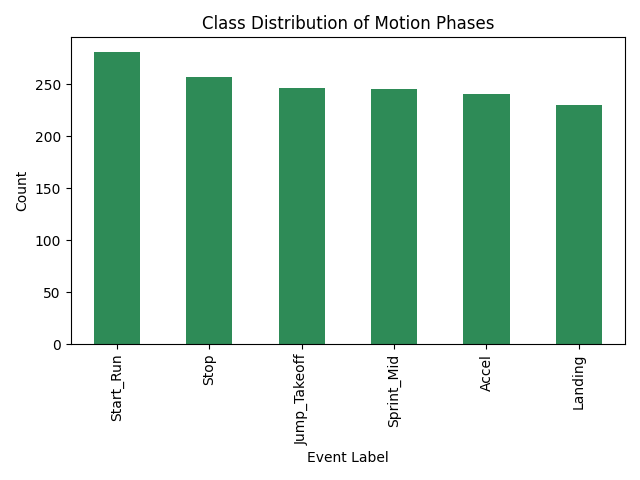
\includegraphics[width=0.85\textwidth]{images/class_distribution_motion_phase.png}
\caption{\textbf{Class distribution of motion phases.} Each of the six
motion phase labels is approximately equally represented across the
1{,}500 records, indicating a balanced dataset with no dominant
class.\label{fig:class-dist}}
\end{figure}



\subsection{Annotated Signal Exploration}
This section characterises the raw sensor signals through time-series
visualisations and annotated event plots, assessing class separability
before feature extraction.

\subsubsection{Signal Plots Around Labeled Events}
Acceleration magnitude ($Acc\_Mag$) and gyroscope magnitude ($Gyro\_Mag$)
were computed as the Euclidean norm of their respective three-axis readings:

\begin{equation}
Acc\_Mag = \sqrt{Acc\_X^2 + Acc\_Y^2 + Acc\_Z^2}
\label{eq:accmag}
\end{equation}

\begin{equation}
Gyro\_Mag = \sqrt{Gyro\_X^2 + Gyro\_Y^2 + Gyro\_Z^2}
\label{eq:gyromag}
\end{equation}

Time-series plots of heart rate, $Acc\_Mag$, and $Gyro\_Mag$ were generated
across the full recording window for all athletes (Figure~\ref{fig:timeseries}).
Box plots grouped by motion phase label were produced to assess raw signal
separability (Figure~\ref{fig:boxplots}). 

\begin{figure}[H]
\centering
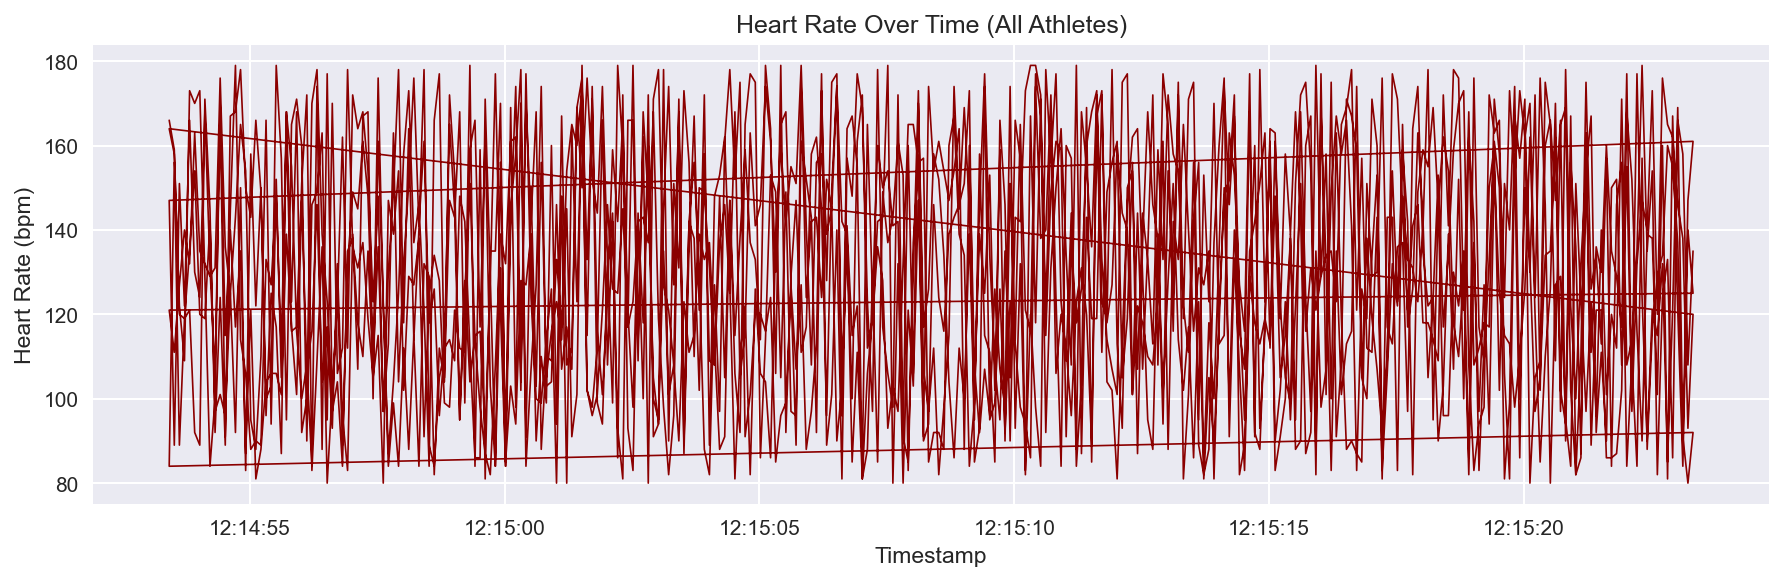
\includegraphics[width=0.65\textwidth]{images/hr_over_time.png}
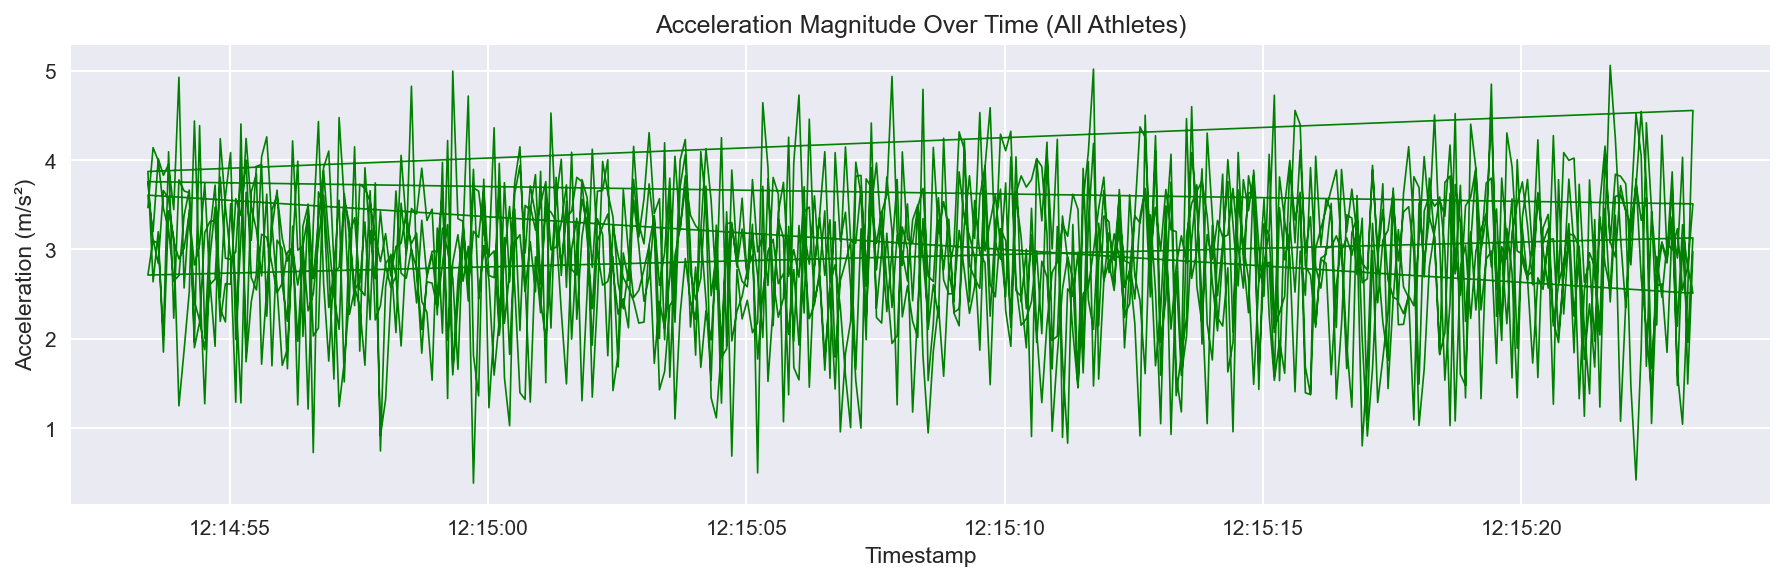
\includegraphics[width=0.65\textwidth]{images/acc_mag_over_time.png}
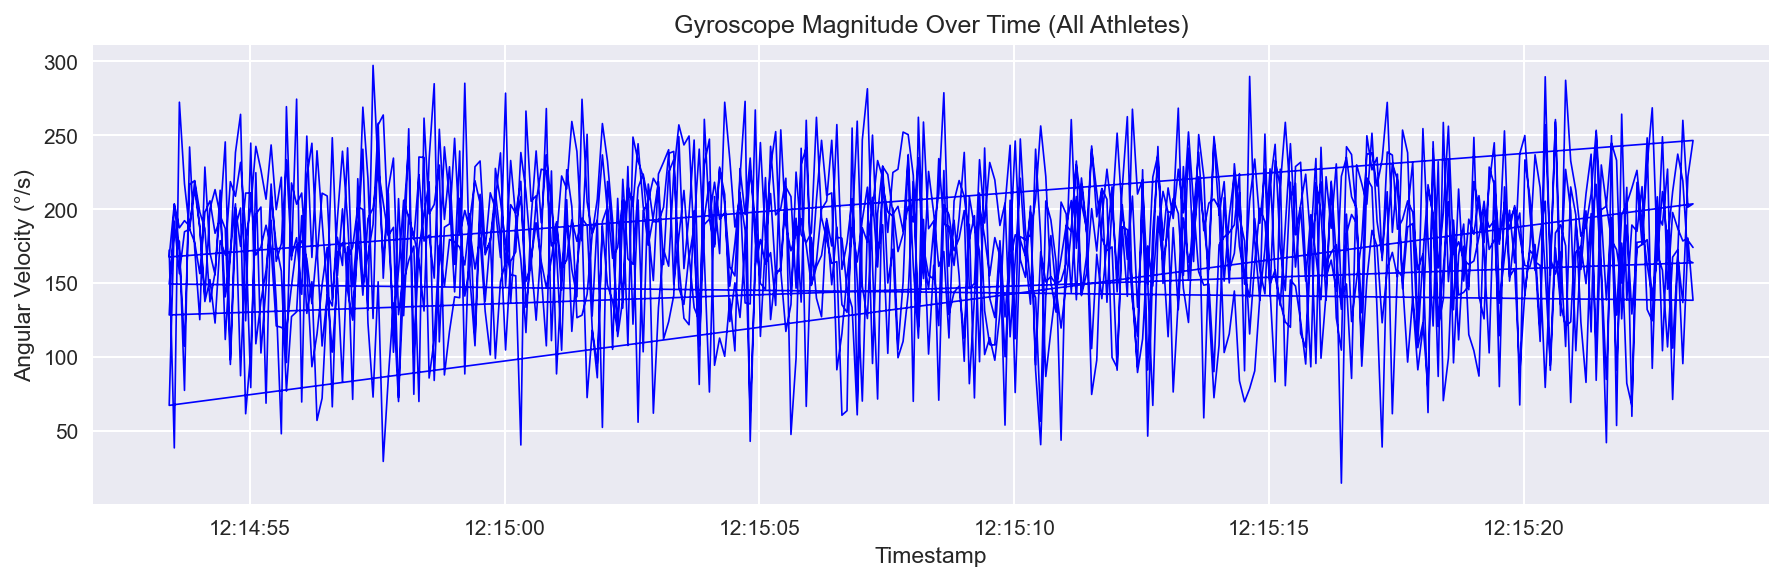
\includegraphics[width=0.65\textwidth]{images/gyro_mag_over_time.png}
\caption{\textbf{Sensor signals over the full recording window.}
Heart rate (top), acceleration magnitude (middle), and gyroscope
magnitude (bottom) across all athletes.\label{fig:timeseries}}
\end{figure}

\begin{figure}[H]
\centering
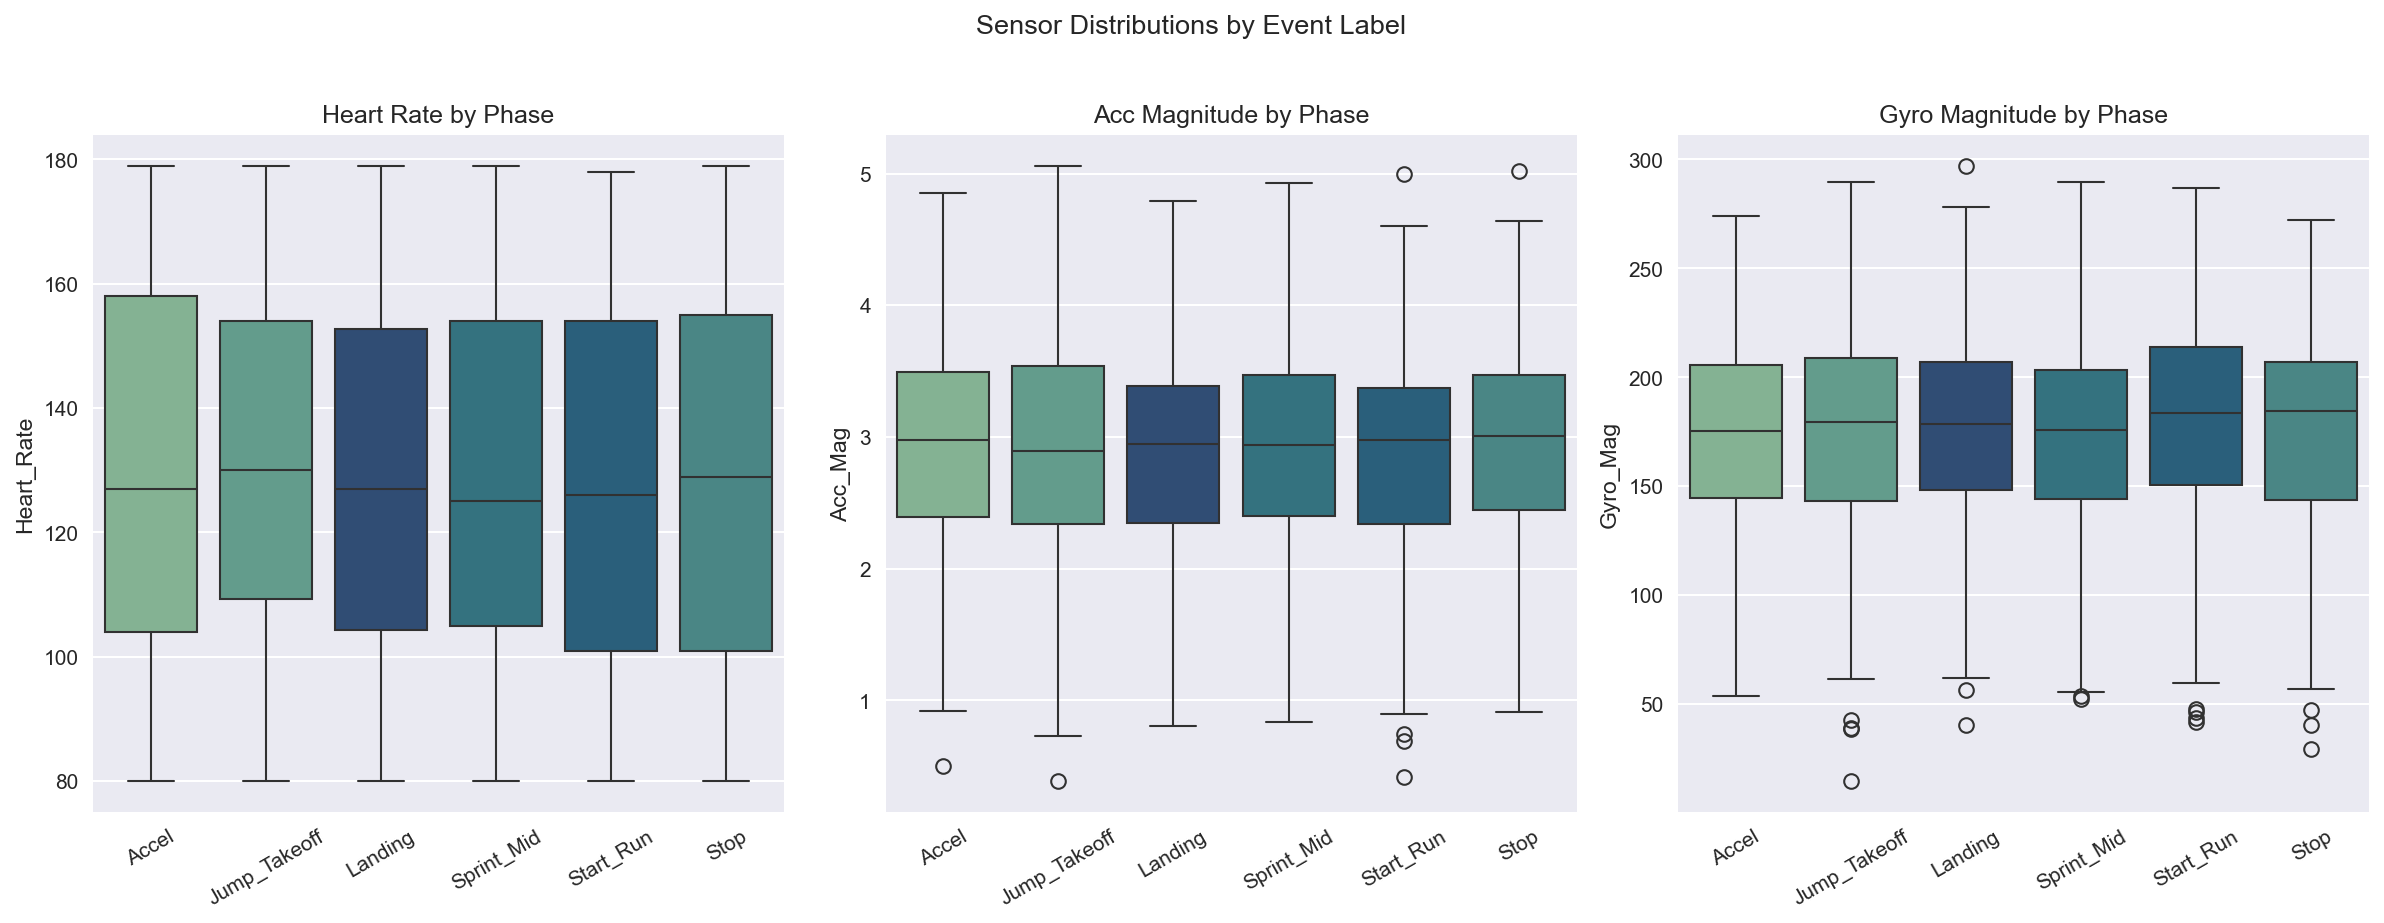
\includegraphics[width=0.95\textwidth]{images/sensor_distributions_by_label.png}
\caption{\textbf{Sensor distributions by motion phase.} Box plots of
heart rate , acceleration magnitude, and gyroscope
magnitude grouped by motion phase label.\label{fig:boxplots}}
\end{figure}

For each of the six motion phase labels, a zoomed
window of 25 samples before and after the event onset was extracted from
Athlete A001 with a dashed vertical line marking the transition point
(Figure~\ref{fig:event-accel}).

\begin{figure}[H]
\centering
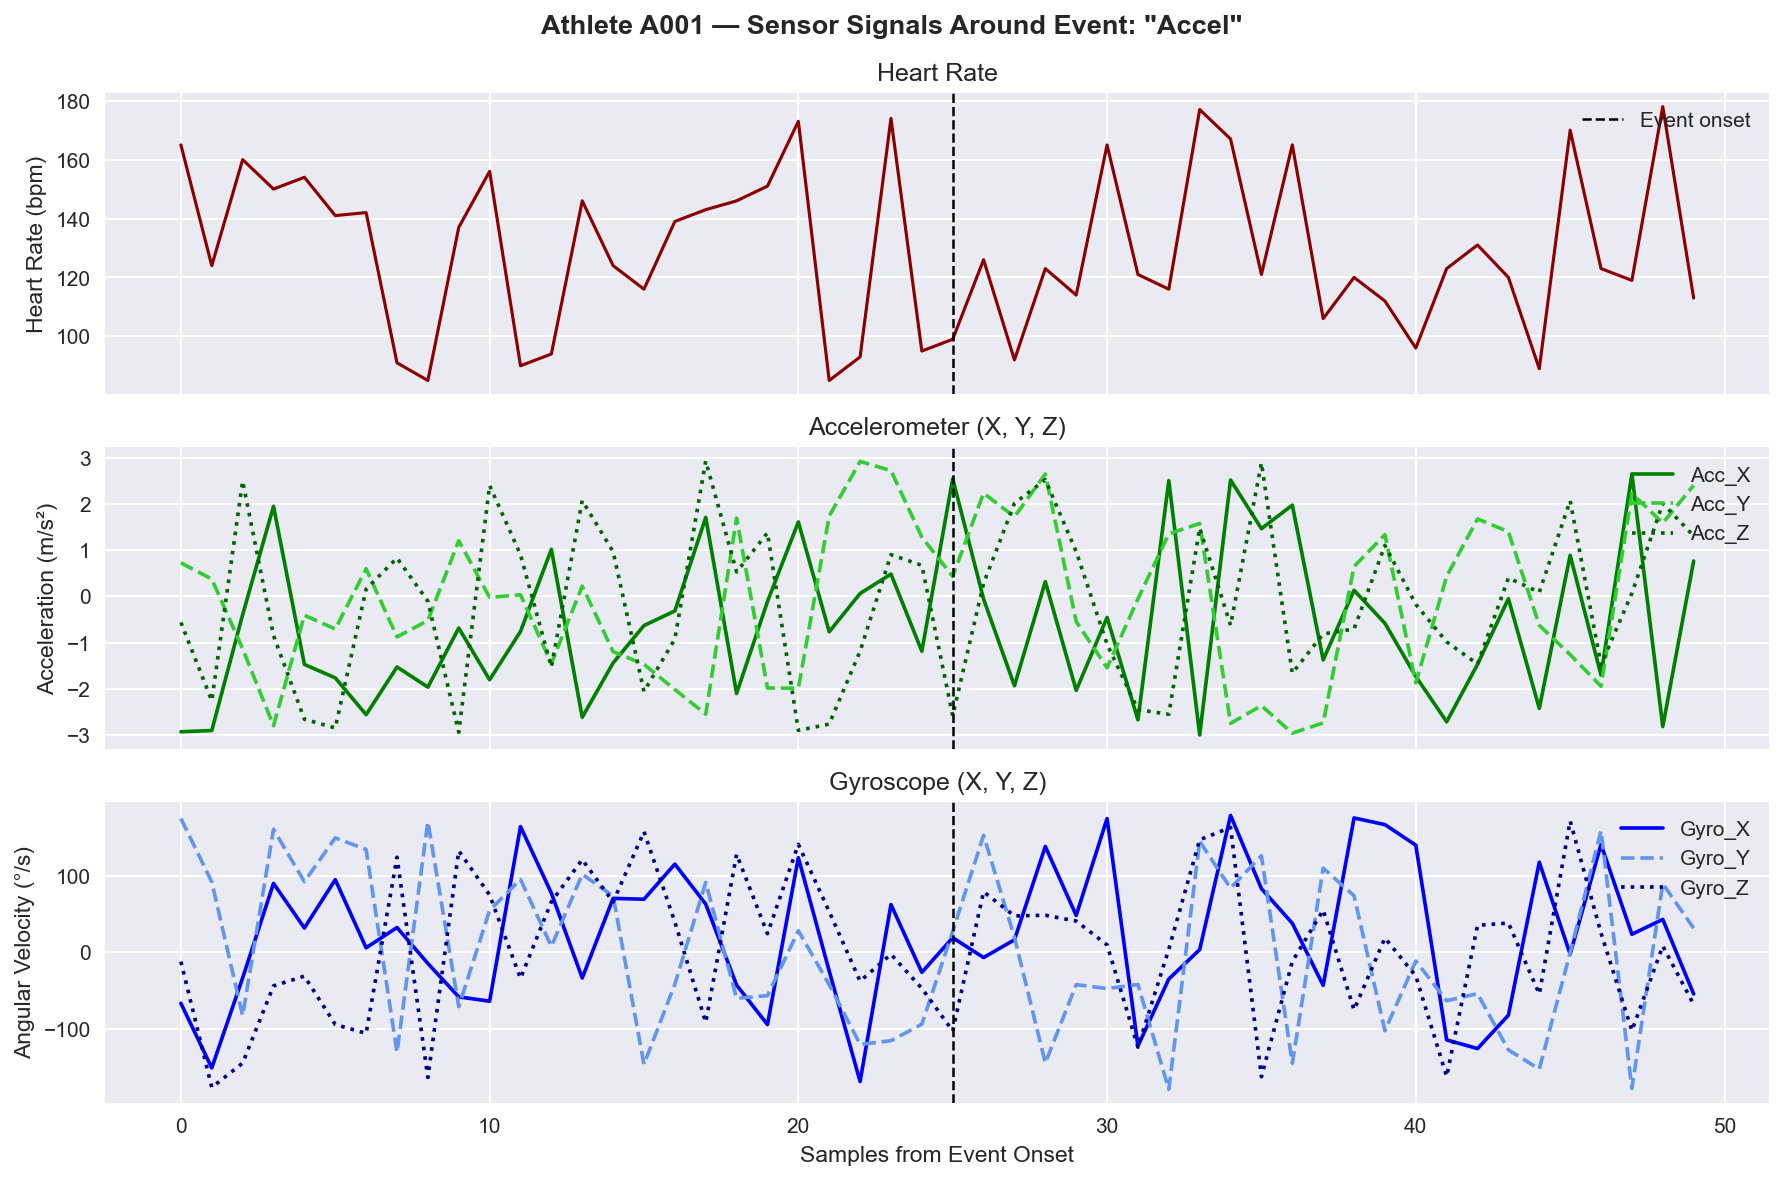
\includegraphics[width=0.9\textwidth]{images/event_signal_A001_Accel.png}
\caption{Sensor signals $\pm$25 samples around an Accel event onset (Athlete A001).\label{fig:event-accel}}
\end{figure}

\begin{figure}[H]
\centering
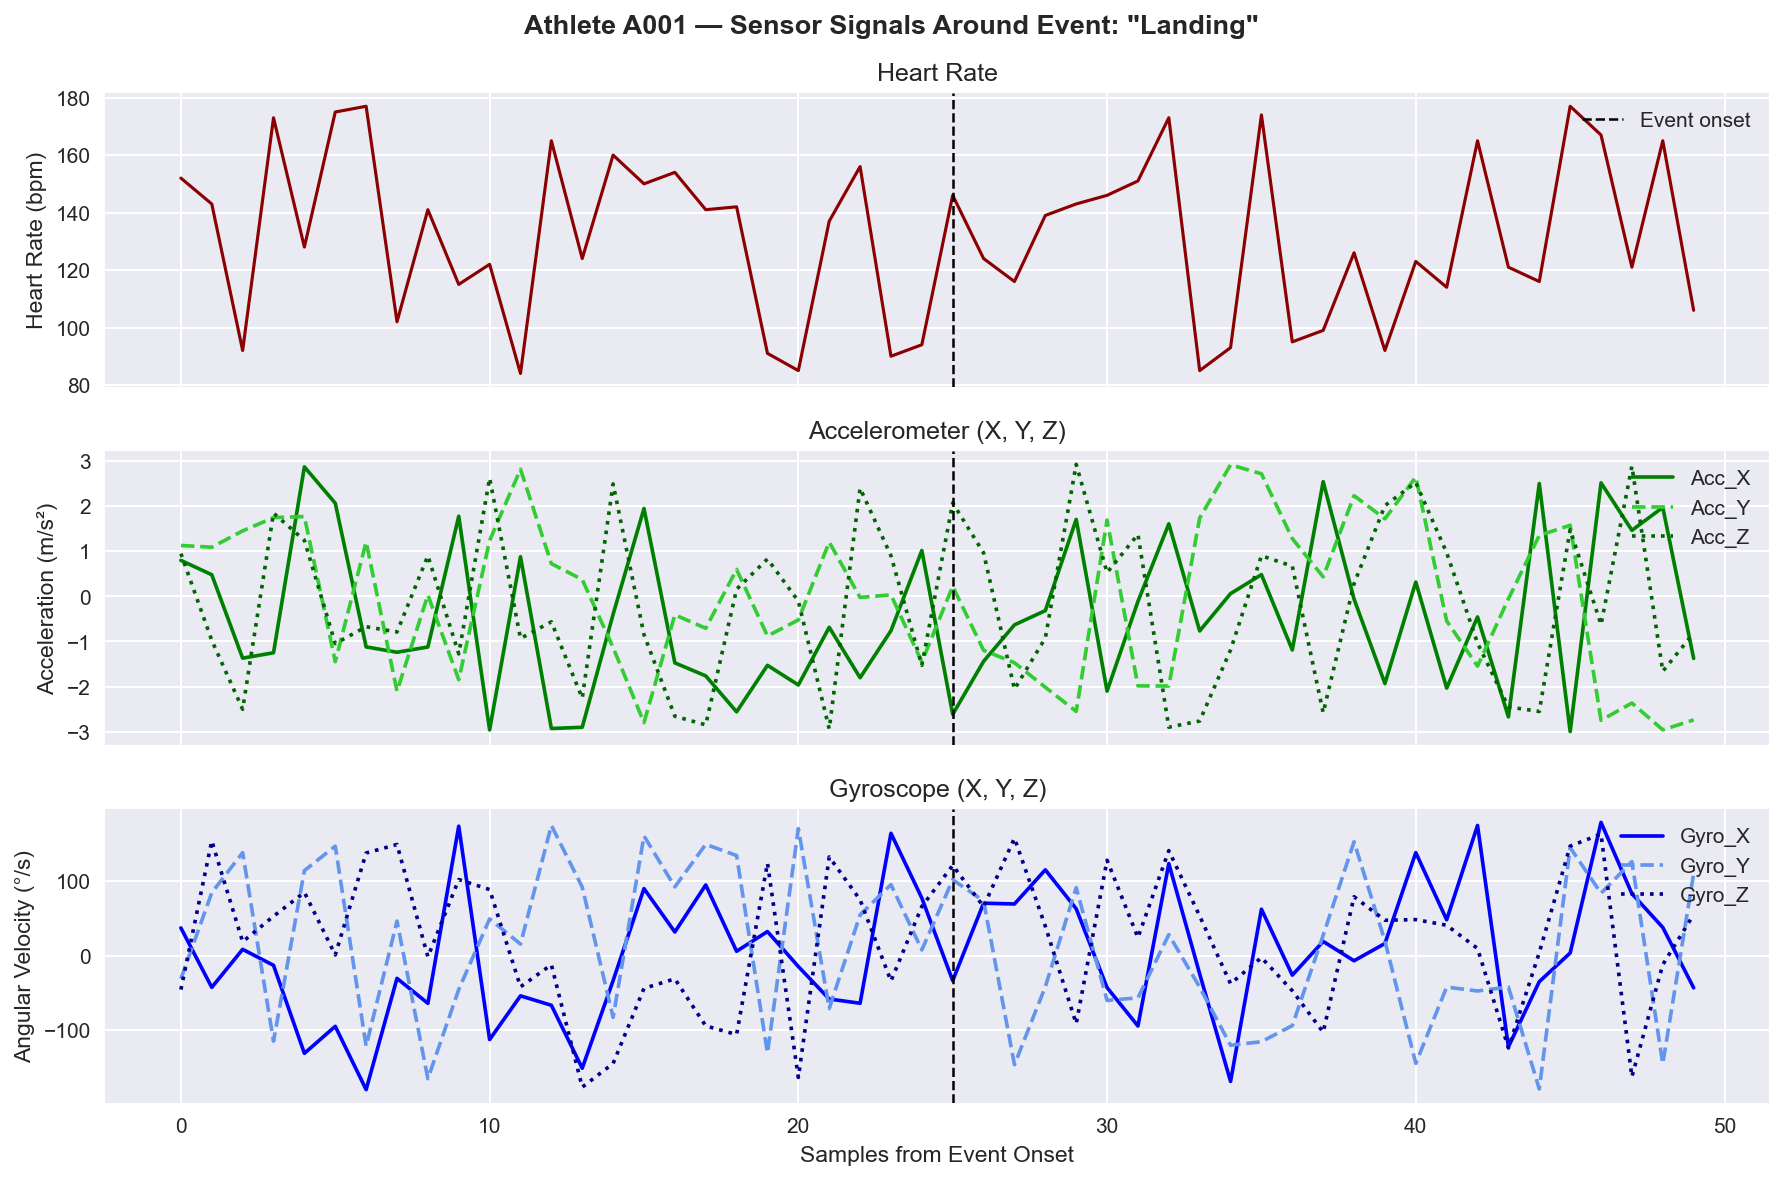
\includegraphics[width=0.9\textwidth]{images/event_signal_A001_Landing.png}
\caption{Sensor signals $\pm$25 samples around a Landing event onset (Athlete A001).\label{fig:event-landing}}
\end{figure}

\subsubsection{Narrative Around Raw Signal Patterns}
Raw signal magnitudes are strikingly similar across all six motion phase classes. Acceleration and gyroscope distributions overlap substantially, confirming that amplitudes alone carry limited discriminative information. Heart rate varies primarily by athlete baseline rather than phase, and responds too slowly to mark individual event boundaries. Accelerometer axes showed the clearest transient responses at event onsets, while gyroscope signals captured rotational changes during direction-change events. These observations confirm that higher-level time-domain and frequency-domain features are necessary for reliable classification.



\subsection{Signal Preprocessing}
\label{sec:PREPROCESSING}
This section describes the preprocessing steps applied to the raw biosensor data prior to windowing and feature extraction.

\subsubsection{Data Cleaning}
Duplicate rows were checked and none were found. Invalid or missing timestamps were also checked and not detected. The data were sorted by \texttt{Athlete\_ID} and time to preserve chronological order. Event labels were standardised to lowercase and a consistent format to eliminate categorical inconsistencies. Since the dataset is already well-formed, no major preprocessing transformations were required.

\subsubsection{Missing Value Findings and Interpolation Strategy}
No missing values were detected across any channel, label, or timestamp column. The dataset is complete as received. Had gaps been present, linear interpolation would have been applied within each athlete's session separately; gaps exceeding five consecutive samples (0.5\,s) would be flagged as sensor dropout rather than interpolated.

\subsubsection{Sampling Rate Confirmation}
Inter-sample intervals were computed per athlete and confirmed to be uniformly 0.1\,s, corresponding to a stable 10\,Hz sampling rate with no gaps or jitter (Table~\ref{tab:sampling_rate}).

\begin{table}[h]
\centering
\begin{tabular}{cc}
\toprule
\textbf{Time Interval (s)} & \textbf{Count} \\
\midrule
0.1 & 1495 \\
\bottomrule
\end{tabular}
\caption{\textbf{Distribution of time intervals between consecutive samples.}}
\label{tab:sampling_rate}
\end{table}

\subsubsection{Filtering Decision}
A low-pass Butterworth filter was considered but rejected. At 10\,Hz the Nyquist frequency is 5\,Hz. Rapid motion transitions (sprint starts, jump landings) occur at timescales that overlap the filter cutoff, and testing confirmed that filtering introduced signal artifacts without reducing noise. Raw signal values are therefore retained for all channels with no filtering applied.

\subsubsection{Per-Athlete Z-Score Normalisation}
To account for inter-athlete baseline differences in heart rate and sensor magnitude, per-athlete z-score normalisation was applied to all seven sensor channels. For each athlete $a$ and channel $c$, the normalised value is:
\begin{equation}
\hat{x}_{a,c} = \frac{x_{a,c} - \mu_{a,c}}{\sigma_{a,c}}
\end{equation}
where $\mu_{a,c}$ and $\sigma_{a,c}$ are the mean and standard deviation computed over all samples from athlete $a$ on channel $c$. This ensures features reflect within-athlete signal variation rather than absolute sensor offsets.

\begin{figure}[H]
\centering
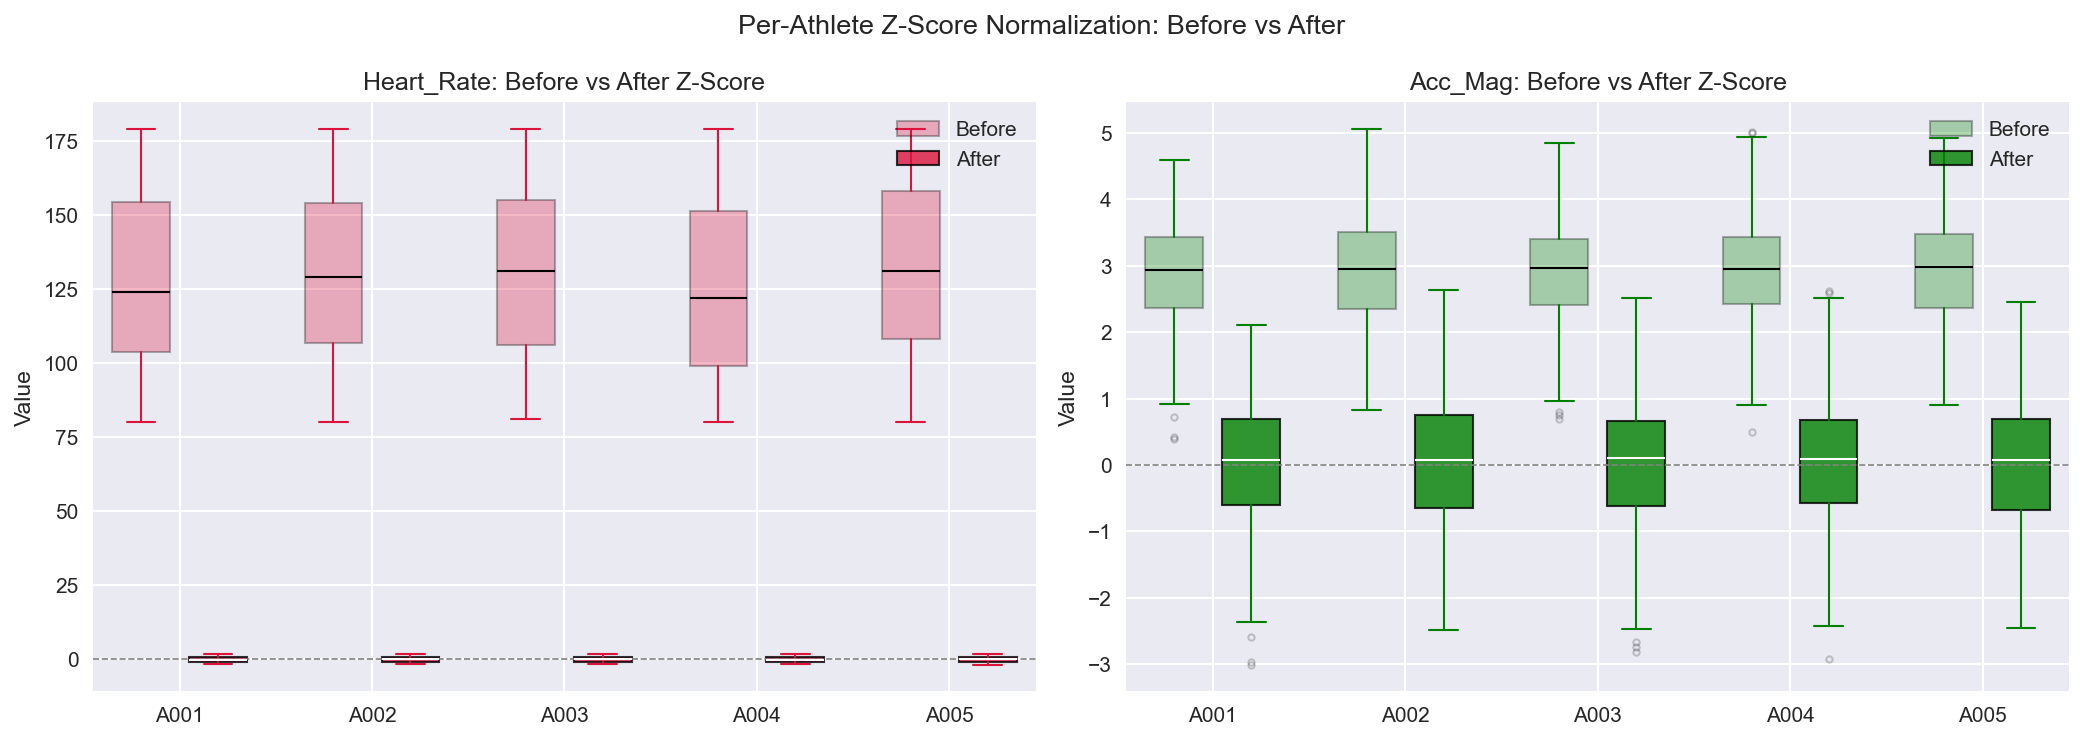
\includegraphics[width=0.99\linewidth]{images/zscore_normalization_comparison.png}
\caption{\textbf{Per-athlete z-score normalisation comparison.} Raw and normalised sensor signals are shown side by side, confirming that inter-athlete baseline differences are removed while within-athlete dynamics are preserved.\label{fig:zscore}}
\end{figure}

\subsubsection{Sensor Range Checks}
Sensor range checks were performed to ensure all values fall within plausible physical limits. Percentile-based outlier detection (1st--99th percentile $+$ 10\% buffer) flagged no raw sensor values as out-of-range; no filtering was applied. Table~\ref{tab:oor-pct} shows the out-of-range rate per channel.

\begin{table}[H]
\centering
\small
\begin{tabular}{lccccccc}
    \toprule
    & \textbf{Heart\_Rate} & \textbf{Acc\_X} & \textbf{Acc\_Y} & \textbf{Acc\_Z} & \textbf{Gyro\_X} & \textbf{Gyro\_Y} & \textbf{Gyro\_Z} \\
    \midrule
    \rowcolor{LightBlue} Out-of-range (\%) & 0.000 & 0.000 & 0.000 & 0.000 & 0.000 & 0.000 & 0.000 \\
    \bottomrule
\end{tabular}
\caption{\textbf{Per-channel out-of-range rate after cleaning.} All sensor readings fall within physically plausible bounds.\label{tab:oor-pct}}
\end{table}


\subsection{Segmentation Strategy}
\label{sec:WINDOWING}
This section describes the sliding window approach used to segment the continuous sensor stream into fixed-length intervals suitable for feature extraction.

\subsubsection{Label Block Structure Analysis}
Consecutive runs of identical labels were analysed per athlete to characterise the temporal structure of the annotations. The median consecutive block length was 1 row (0.1\,s) and the maximum was 6 rows (0.6\,s). Labels transition nearly every row, meaning any window longer than 0.1\,s will span multiple event types and receive a noisy majority label. This rapid label switching is the primary source of label noise throughout the pipeline.

\subsubsection{Sliding Window Sweep}
A unified window size sweep was conducted using the tuned Random Forest with the top 20 consensus-selected features, evaluated under both Stratified 5-Fold CV and LOSO CV~\cite{10962074}. Ten window sizes from 0.2\,s to 2.0\,s in 0.2\,s steps were evaluated~\cite{10689691}. For each window size, average label purity was also recorded as a measure of label noise introduced by the sliding window. Full sweep results are reported in Section~\ref{sec:results_discussion}.

\subsubsection{Window Size Selection and Justification}
$W = 1.0$\,s was selected for three reasons: (a) it exceeds the maximum observed label block length (0.6\,s), ensuring each window can capture at least one complete phase; (b) it yields 580 windows (116 per athlete), the largest stable sample count before per-class windows become too few to support reliable CV; (c) label purity at 1.0\,s (0.344) offers the best purity--sample-count trade-off across all sizes tested. The label assigned to each window is determined by majority vote over the event labels of its samples. The full configuration is summarised in Table~\ref{tab:window-config}.

\begin{table}[H]
\centering
\small
\begin{tabularx}{0.45\textwidth}{lX}
    \toprule
    \textbf{Parameter} & \textbf{Value} \\
    \midrule
    \rowcolor{LightBlue} Window size & 1.0 s \\
    Step ratio & 0.25 \\
    \rowcolor{LightBlue} Step size & 0.25 s \\
    Min.\ samples per window & 1 \\
    \rowcolor{LightBlue} Total windows generated & 580 \\
    \bottomrule
\end{tabularx}
\caption{\textbf{Sliding window configuration.} Parameters used for segmentation throughout training and evaluation.\label{tab:window-config}}
\end{table}

\subsection{Feature Engineering}
\label{sec:FEATURES}
This section describes the extraction, ranking, and selection of features from the segmented biosensor windows.

\subsubsection{Feature Extraction: Time Domain}
For each of the 7 raw sensor channels (Heart\_Rate, Acc\_X/Y/Z, Gyro\_X/Y/Z), four time-domain features were extracted per window: mean, standard deviation, root mean square (RMS), and zero-crossing rate (ZCR). This yields $7 \times 4 = 28$ time-domain features.

\subsubsection{Feature Extraction: Frequency Domain}
Three frequency-domain features were derived per channel via the real FFT of the mean-centred window samples: dominant frequency (Hz), spectral energy, and spectral entropy. This yields $7 \times 3 = 21$ frequency-domain features. Additionally, eight cross-axis Pearson correlation coefficients were computed: \texttt{Acc\_XY}, \texttt{Acc\_XZ}, \texttt{Acc\_YZ}, \texttt{Gyro\_XY}, \texttt{Gyro\_XZ}, \texttt{Gyro\_YZ}, \texttt{AccMag\_GyroMag}, and \texttt{HR\_AccMag}. Combined with the 49 per-channel descriptors, this yields a total of 57 features per window.

\begin{table}[H]
\caption{\textbf{Summary of extracted features.} Features built from 1.0\,s sliding windows with a 0.25 step ratio.}
\label{tab:feature_summary}
\small
\centering
\begin{tabularx}{0.95\textwidth}{l l X}
\toprule
\textbf{Source} & \textbf{Feature type} & \textbf{Extracted features} \\
\midrule
Heart rate, accelerometer, gyroscope & Time-domain & Mean, standard deviation, RMS, zero-crossing rate \\
\rowcolor{LightBlue}
Heart rate, accelerometer, gyroscope & Frequency-domain & Dominant frequency, spectral energy, spectral entropy \\
Accelerometer, gyroscope & Engineered & Acceleration magnitude, gyroscope magnitude, 8 axis-pair correlations \\
\bottomrule
\end{tabularx}
\end{table}

\subsubsection{Feature Ranking (MI + ANOVA + RF Importance)}
Features were ranked using three complementary criteria computed on a training-athlete subset: mutual information (non-linear class dependence), ANOVA $F$-statistic (linear separability), and Random Forest importance. Each criterion is normalised to $[0,1]$ and averaged into a consensus score; the top $K = 20$ features are identified. Pairwise Pearson correlations were also checked among the top 20; no pairs exceeded $r > 0.95$, so all 20 were retained.

\begin{figure}[H]
\centering
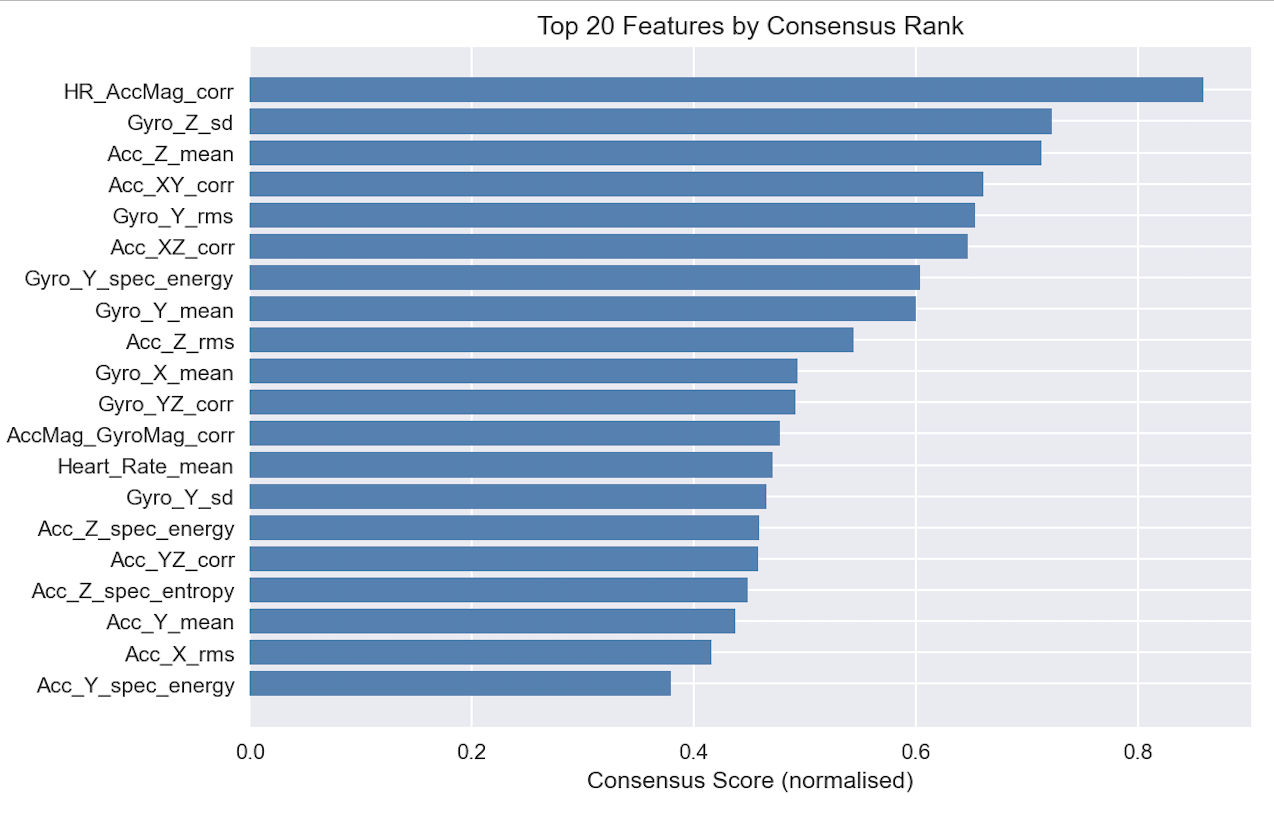
\includegraphics[width=0.9\textwidth]{images/feature_ranking.png}
\caption{\textbf{Top-ranked features by consensus score.} \texttt{HR\_AccMag\_corr} ranks highest, followed by \texttt{Gyro\_Z\_sd} and \texttt{Acc\_Z\_mean}.\label{fig:feature_importance}}
\end{figure}

\subsubsection{Feature Selection and Interpretation}
The final selected feature count is 20. \texttt{SelectKBest} (mutual information scoring) is applied inside each CV fold with $k$ searched over $\{15, 20, 25\}$ during tuning to prevent cross-fold leakage. \texttt{HR\_AccMag\_corr} ranks highest, capturing the coupling between cardiovascular load and movement intensity across phases. Sagittal gyroscope features (\texttt{Gyro\_Z\_sd}, \texttt{Gyro\_Y} family) distinguish sprint and acceleration phases from stationary ones. Vertical-axis acceleration (\texttt{Acc\_Z\_mean}, \texttt{Acc\_Z\_rms}) reflects loading patterns for \textit{jump\_takeoff} and \textit{landing}. Cross-axis correlations (\texttt{Acc\_XY\_corr}, \texttt{Acc\_XZ\_corr}) suggest phase transitions involve multi-axis coupling rather than single-axis signals alone.




\subsection{Modeling}
\label{sec:MODEL}
This section describes the train/test setup, baseline evaluation, hyperparameter tuning, and deep learning extension.

\subsubsection{Train/Test Split and Cross-Validation Setup}
The dataset was split 80/20 stratified by class (\texttt{random\_state=42}), yielding 464 training and 116 test samples. A \texttt{StandardScaler} was fit on the training set only and applied to both splits to prevent data leakage. Two cross-validation strategies were used: Stratified 5-Fold CV for hyperparameter tuning, where windows from the same athlete can appear in both train and test folds producing an optimistic estimate; and Leave-One-Athlete-Out (LOSO) CV, where each fold holds out one athlete entirely with the scaler refit per fold, giving a realistic cross-subject generalisation estimate.

\subsubsection{Baseline Results (Dummy and Pre-Tuning)}
A \texttt{DummyClassifier} (most-frequent strategy) establishes the performance floor: 5-Fold accuracy $0.222 \pm 0.003$, LOSO accuracy $0.179 \pm 0.044$, against a uniform chance level of $0.167$. Table~\ref{tab:pretune} shows all seven classifiers at default settings before tuning; all real models must exceed the dummy baseline.

\begin{table}[H]
\centering
\small
\csvautotabular{csvFiles/baselineScores.csv}
\caption{\textbf{Pre-tuning baseline results.} All seven classifiers at default settings.\label{tab:pretune}}
\end{table}

\subsubsection{Hyperparameter Tuning}
Each model was tuned with \texttt{GridSearchCV} (5-fold stratified CV), searching over model-specific grids plus \texttt{selector\_\_k} $\in \{15,20,25\}$ features; best parameters were selected by macro-averaged accuracy. Table~\ref{tab:tuning} summarises the best configuration and CV accuracy per model.

\begin{table}[H]
\centering
\small
\begin{tabularx}{\textwidth}{lcX}
\toprule
\textbf{Model} & \textbf{Best CV Acc} & \textbf{Best Parameters} \\
\midrule
\rowcolor{LightBlue} Random Forest & 0.3039 & {\footnotesize\texttt{n\_estimators=300, max\_depth=None, min\_samples\_leaf=1, class\_weight="balanced"}} \\
XGBoost       & 0.2888 & {\footnotesize\texttt{n\_estimators=400, max\_depth=3, learning\_rate=0.2, subsample=0.7}} \\
\rowcolor{LightBlue} SVM-RBF       & 0.2866 & {\footnotesize\texttt{C=10, gamma="scale", class\_weight="balanced"}} \\
Decision Tree & 0.2348 & {\footnotesize\texttt{max\_depth=15, min\_samples\_leaf=1, criterion="gini"}} \\
\rowcolor{LightBlue} Naive Bayes   & 0.2306 & {\footnotesize\texttt{var\_smoothing=$10^{-11}$}} \\
AdaBoost      & 0.2241 & {\footnotesize\texttt{n\_estimators=200, learning\_rate=0.01}} \\
\bottomrule
\end{tabularx}
\caption{Best hyperparameters and 5-Fold CV accuracy per model after \texttt{GridSearchCV}.\label{tab:tuning}}
\end{table}

Figure~\ref{fig:pretuning_vs_posttuning} compares pre-tuning and post-tuning CV accuracy for all models, showing the improvement gained from \texttt{GridSearchCV}.

\begin{figure}[H]
\centering
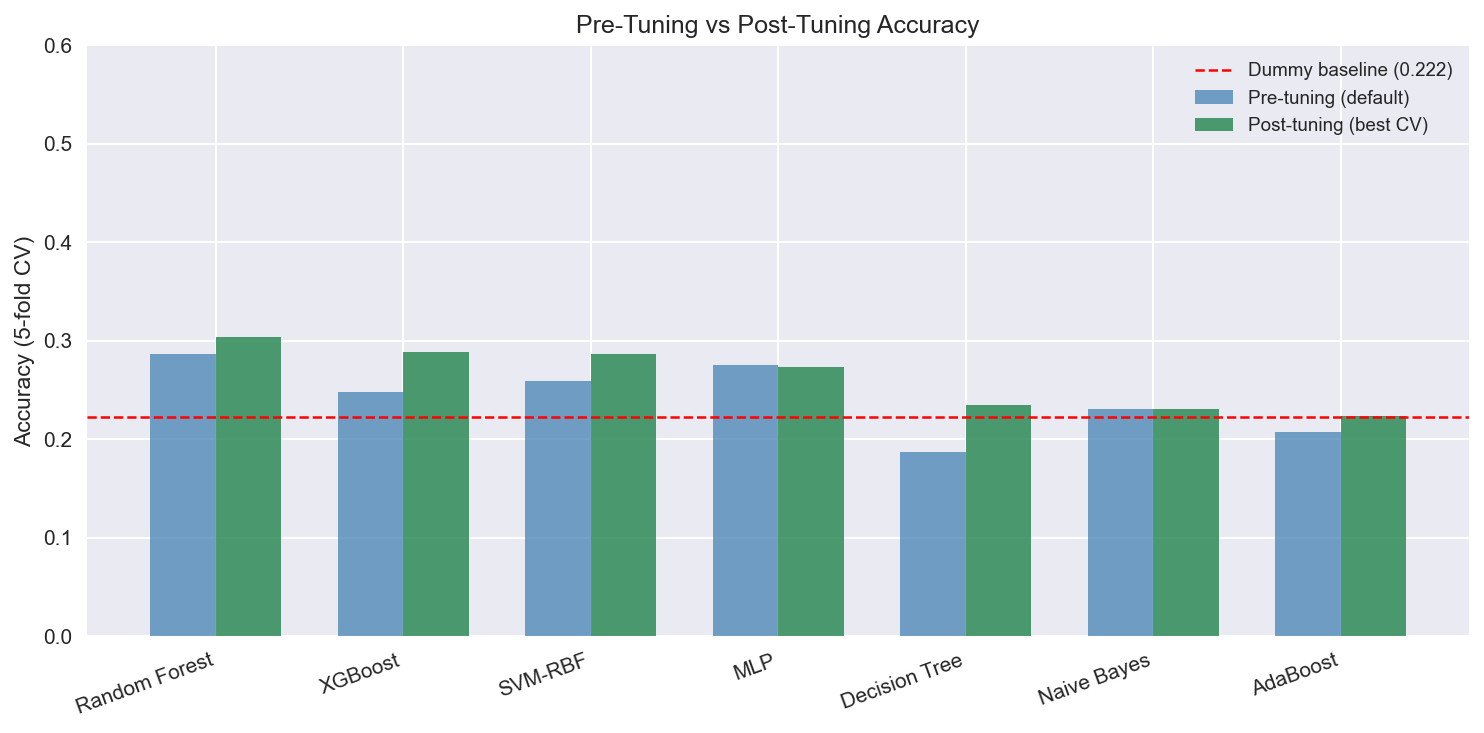
\includegraphics[width=0.95\linewidth]{images/pretuning_vs_posttuning.png}
\caption{Pre-tuning vs.\ post-tuning 5-Fold CV accuracy for all seven models.}
\label{fig:pretuning_vs_posttuning}
\end{figure}

Table~\ref{tab:model_results} summarises tuned 5-Fold CV and LOSO accuracy for all seven models.

\begin{table}[H]
\centering
\small
\caption{\textbf{Tuned model accuracy under 5-Fold CV and LOSO CV.}\label{tab:model_results}}
\begin{tabular}{lcccc}
\toprule
\textbf{Model} & \textbf{5-Fold Acc} & \textbf{5-Fold Std} & \textbf{LOSO Acc} & \textbf{LOSO Std} \\
\midrule
\rowcolor{LightBlue} Random Forest & 0.3039 & 0.0590 & 0.1811 & 0.0585 \\
XGBoost       & 0.2888 & 0.0234 & 0.2056 & 0.0414 \\
\rowcolor{LightBlue} SVM-RBF       & 0.2866 & 0.0530 & 0.1755 & 0.0502 \\
MLP           & 0.2738 & 0.0416 & 0.1898 & 0.0159 \\
\rowcolor{LightBlue} Decision Tree & 0.2348 & 0.0727 & 0.1896 & 0.0422 \\
Naive Bayes   & 0.2306 & 0.0498 & 0.1396 & 0.0332 \\
\rowcolor{LightBlue} AdaBoost      & 0.2241 & 0.0183 & 0.1596 & 0.0521 \\
\bottomrule
\end{tabular}
\end{table}

\subsubsection{Deep Learning Extension}

\paragraph{Input Reshaping.} To prepare data for sequence-based architectures, raw sensor windows were reshaped into 3D tensors of shape \texttt{(n\_windows, 50, 9)}, where 50 timesteps were obtained by resampling each window via linear interpolation, and 9 channels correspond to Heart Rate, Acc X/Y/Z, Gyro X/Y/Z, Acc Magnitude, and Gyro Magnitude. The resulting tensors were saved as \texttt{X\_sequences.npy} and \texttt{y\_sequences.npy}, ready for LSTM, GRU, or Conv1D architectures.

\paragraph{ANN Architecture.} As a deep learning baseline, a feedforward Artificial Neural Network (ANN) was trained directly on the scaled 20-feature matrix (input shape $(N, 20)$), where each row represents one segmented window described by its extracted features. Unlike the classical models, the ANN learns non-linear combinations of features through multiple hidden layers rather than relying on hand-crafted decision boundaries.

The network uses two hidden blocks, each consisting of a fully-connected (Dense) layer followed by Batch Normalisation and Dropout. Batch Normalisation stabilises training by normalising activations within each mini-batch, reducing sensitivity to weight initialisation. Dropout randomly deactivates 30\% of neurons during training, which acts as a regulariser to prevent overfitting on the small dataset. The final layer outputs a probability distribution over the six motion-phase classes using a Softmax activation. Table~\ref{tab:ann} summarises the layer stack.

\begin{table}[H]
\centering
\small
\begin{tabular}{cll}
\toprule
\textbf{Layer} & \textbf{Type} & \textbf{Details} \\
\midrule
1 & Dense        & 128 units, ReLU activation \\
2 & BatchNorm    & normalises layer activations \\
3 & Dropout      & rate = 0.3 \\
4 & Dense        & 64 units, ReLU activation \\
5 & BatchNorm    & normalises layer activations \\
6 & Dropout      & rate = 0.3 \\
7 & Dense        & 6 units, Softmax (one per class) \\
\bottomrule
\end{tabular}
\caption{ANN layer stack.\label{tab:ann}}
\end{table}

\noindent The model was compiled with the Adam optimiser (learning rate $10^{-3}$) and sparse categorical cross-entropy loss, which is standard for multi-class classification with integer labels. Training ran for up to 25 epochs with a batch size of 32 and a 20\% validation split held out from the training set. Early stopping (patience = 10, \texttt{restore\_best\_weights=True}) halted training if validation loss did not improve for 10 consecutive epochs and restored the weights from the best epoch, preventing the model from overfitting to the training data.

\begin{figure}[H]
\centering
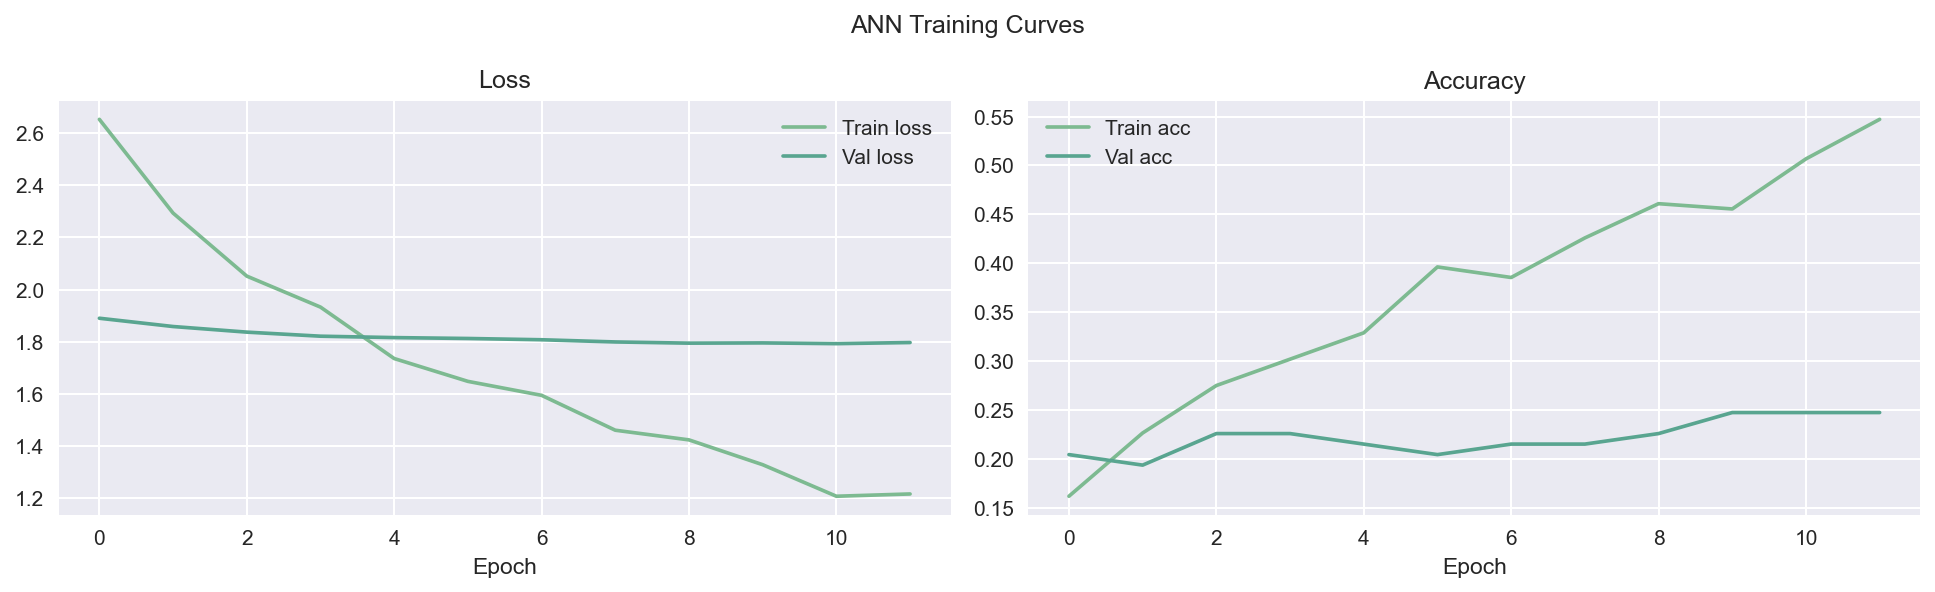
\includegraphics[width=0.95\linewidth]{images/ann_training_curves.png}
\caption{ANN training and validation loss/accuracy curves over epochs. Early stopping halts training when validation loss stops improving.}
\label{fig:ann_training_curves}
\end{figure}



\section{Results \& Discussion}
\label{sec:results_discussion}
This section consolidates the full motion phase classification results and their interpretation. It begins with held-out test-set performance after tuning, then compares the ANN against classical models, followed by cross-validation results under both standard and LOSO protocols. It then analyses window size effects, per-class metrics, confusion matrices, error patterns, and system integration before closing with a synthesis of the main limitations and takeaways.

\subsection{Post-Tuning Test Set Results}
After hyperparameter tuning, each model was evaluated on the held-out 20\% test set (116 windows) that was never seen during training or cross-validation. Table~\ref{tab:testresults} reports accuracy, macro-averaged precision, recall, and F1-score. MLP achieved the highest test accuracy (0.319), closely followed by SVM-RBF (0.310). Notably, SVM-RBF edges out MLP on F1-macro (0.313 vs.\ 0.312), suggesting its per-class predictions are slightly more balanced. AdaBoost stands out with a very low precision (0.081) despite reasonable recall, indicating it over-predicts a single majority class.

\begin{table}[H]
\centering
\small
\begin{tabular}{lcccc}
\toprule
\textbf{Model} & \textbf{Accuracy} & \textbf{Precision} & \textbf{Recall} & \textbf{F1-macro} \\
\midrule
\rowcolor{LightBlue} MLP           & 0.319 & 0.329 & 0.306 & 0.312 \\
SVM-RBF       & 0.310 & 0.311 & 0.315 & 0.313 \\
\rowcolor{LightBlue} XGBoost       & 0.302 & 0.296 & 0.291 & 0.286 \\
Random Forest & 0.267 & 0.255 & 0.246 & 0.246 \\
\rowcolor{LightBlue} Naive Bayes   & 0.259 & 0.260 & 0.250 & 0.254 \\
AdaBoost      & 0.241 & 0.081 & 0.185 & 0.112 \\
\rowcolor{LightBlue} Decision Tree & 0.207 & 0.210 & 0.218 & 0.211 \\
\bottomrule
\end{tabular}
\caption{Held-out test set performance for all tuned models, sorted by accuracy.\label{tab:testresults}}
\end{table}

\begin{figure}[H]
\centering
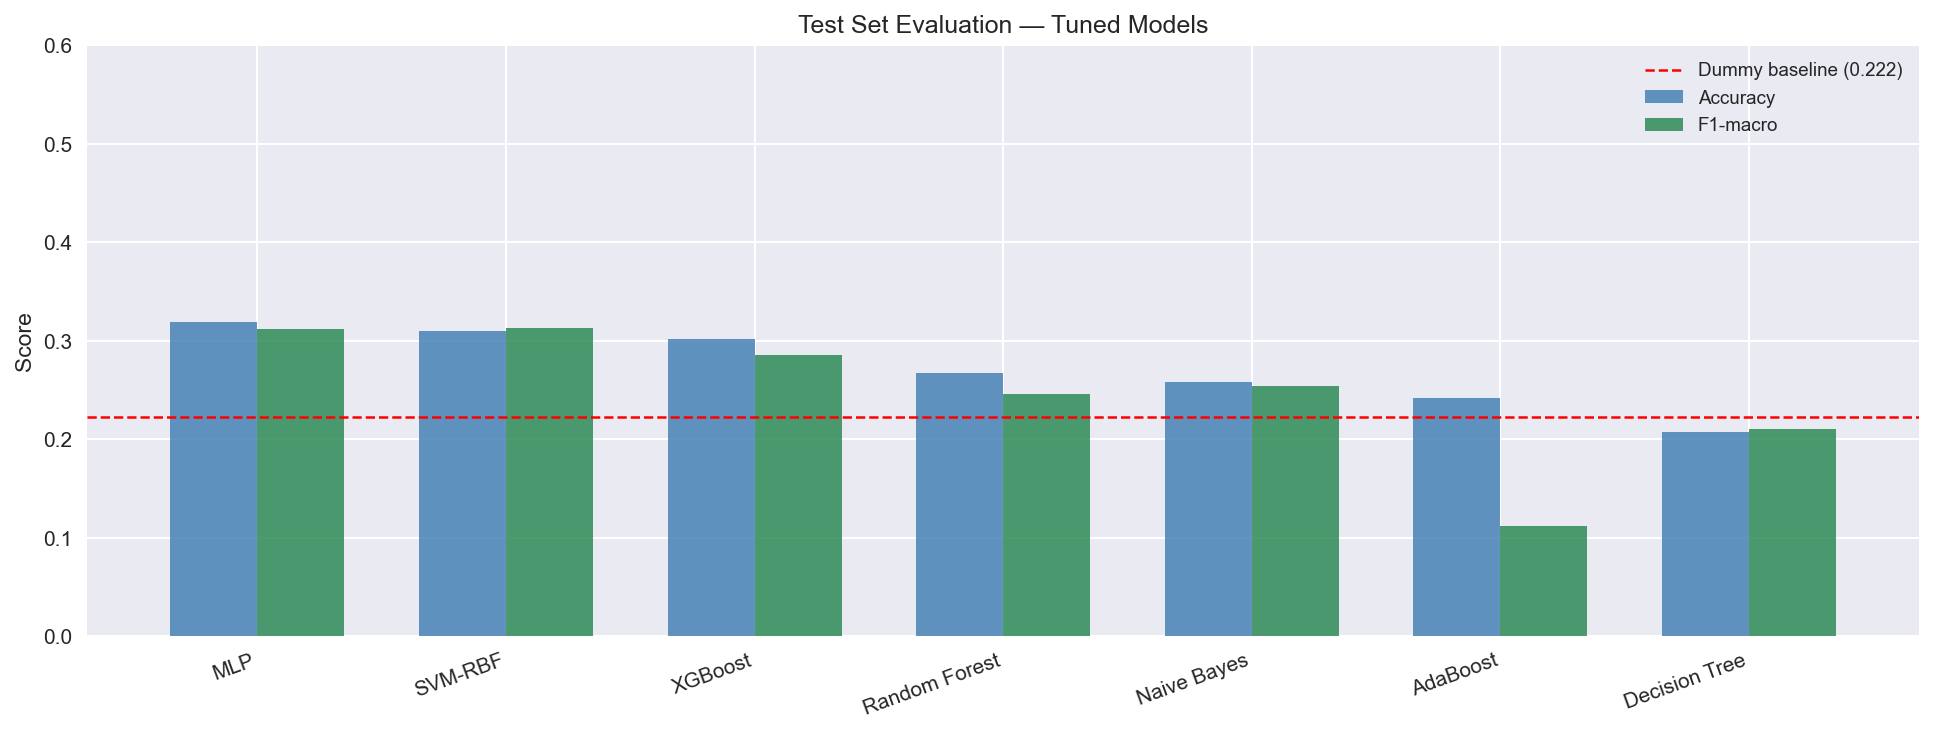
\includegraphics[width=0.95\linewidth]{images/test_set_evaluation.png}
\caption{Test set accuracy, precision, recall, and F1-macro for all tuned models.}
\label{fig:test_set_evaluation}
\end{figure}

\subsection{ANN vs Classical Model Comparison}
The feedforward ANN (MLP) achieved the highest test accuracy (0.319) among all models, outperforming the best classical model (SVM-RBF, 0.310) by approximately one percentage point. However, the margin is narrow and SVM-RBF achieves a marginally higher F1-macro (0.313 vs.\ 0.312), meaning their overall class-balance is comparable. This suggests that for a dataset of this size (580 windows, 20 features), a well-tuned classical model is competitive with a feedforward neural network. The ANN's advantage would be expected to grow with more data, since deep models typically require larger training sets to outperform classical approaches \cite{Mekruksavanich2026}.

\subsection{Standard Split Evaluation: All Models}
Under stratified 5-Fold cross-validation, all models exceed the dummy classifier baseline of 0.222. Random Forest achieved the highest 5-Fold CV accuracy (0.304), though this is an optimistic estimate since windows from the same athlete can appear in both training and test folds. Table~\ref{tab:model_results} shows the full 5-Fold results alongside LOSO for all seven models.

\begin{equation}
\text{CV Mean Difference} = \text{Mean}_{5\text{-Fold}} - \text{Mean}_{\text{LOSO}}
\end{equation}

A positive value indicates 5-Fold outperforms LOSO for that model. All models show a positive gap, confirming that within-fold athlete overlap inflates 5-Fold estimates.

\subsection{LOSO Evaluation: All Models}
Under Leave-One-Athlete-Out (LOSO) cross-validation, each fold holds out one of the five athletes entirely, and the scaler is refit on the remaining four. This is the more realistic evaluation since it directly tests generalisation to an unseen subject. LOSO accuracy is substantially lower for all models; XGBoost achieved the best LOSO score (0.206), only marginally above the six-class chance level of 0.167. This confirms that the models are largely learning athlete-specific patterns rather than generalisable motion signatures. Table~\ref{tab:model_results} summarises both CV strategies for all seven models.

\subsection{Window Size Comparison}

A unified window size sweep was conducted using the tuned Random Forest with the top 20 consensus-selected features, evaluated under both stratified 5-fold CV and LOSO CV~\cite{10962074}. Ten window sizes from 0.2\,s to 2.0\,s in 0.2\,s increments were tested~\cite{10689691}, and label purity was recorded for each size.

\subsubsection{Standard Split Sweep}
Under 5-Fold CV, accuracy rises steadily from near-chance (0.15 at 0.2\,s) to a peak of approximately 0.39 at 1.6\,s. The upward trend with window size is expected: larger windows capture more context per sample, but they also increase the chance that a single athlete's patterns dominate a fold.

\subsubsection{LOSO Sweep}
Under LOSO, accuracy stays near chance (0.15--0.21) at every window size regardless of how large the window is. This flat LOSO curve, while the 5-Fold curve rises, is the key diagnostic: the models are memorising per-athlete patterns rather than learning transferable motion features. High variance at larger windows (e.g., $\pm$0.07 at 1.4\,s) also reflects instability from the reduced number of windows per class at larger sizes.

\subsubsection{Purity Analysis and Justification}
For each window size, label purity was recorded as the fraction of timesteps in a window that share the majority label. At $W = 1.0$\,s, purity is 0.344, the best balance between purity and sample count across all tested sizes. This window also exceeds the maximum observed label block length (0.6\,s), yielding 580 windows (116 per athlete). Table~\ref{tab:window_sizes} and Figure~\ref{fig:windowSizesPNG} summarise the full sweep.

\begin{table}[H]
\centering
\csvautotabular{csvFiles/windowSizeComparison.csv}
\caption{Accuracy and label purity across window sizes (tuned Random Forest).}
\label{tab:window_sizes}
\end{table}

\begin{figure}[H]
\centering
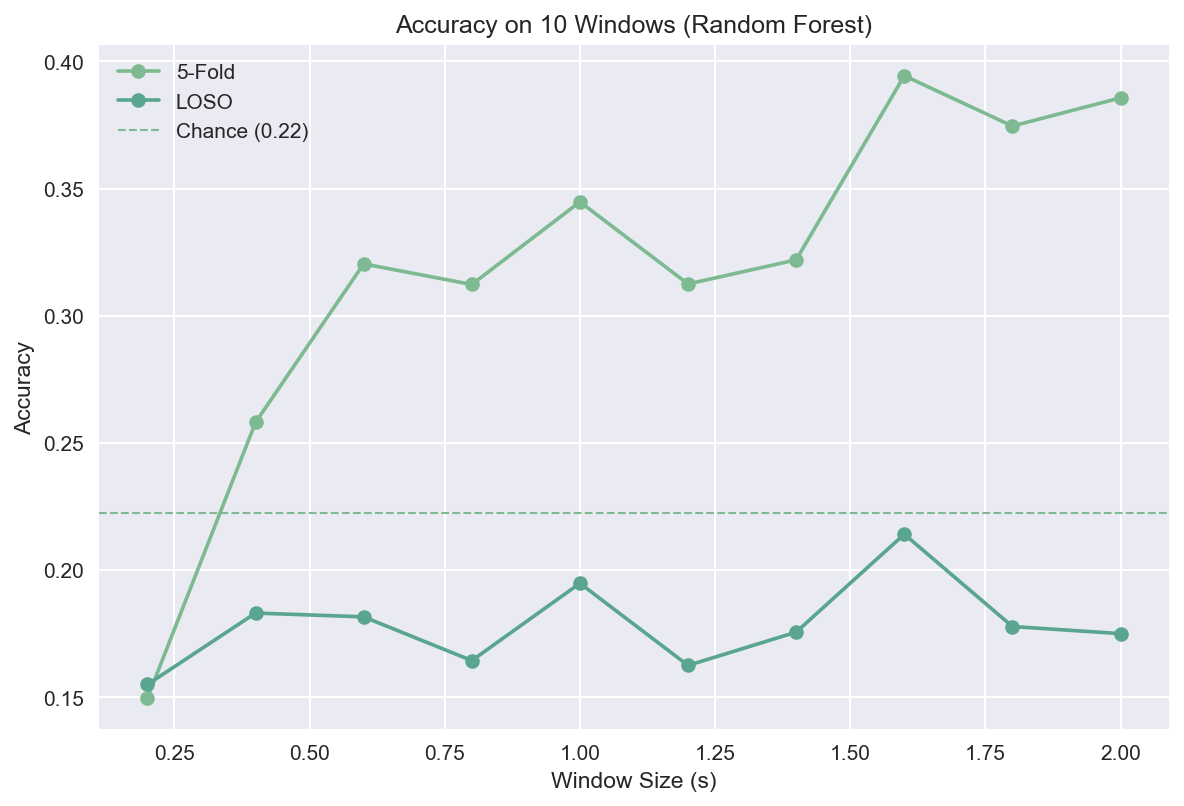
\includegraphics[width=0.9\linewidth]{images/window_size_comparison.png}
\caption{Tuned Random Forest accuracy across 10 window sizes under 5-Fold CV and LOSO CV. The dashed line marks the six-class chance baseline ($\approx$0.167).}
\label{fig:windowSizesPNG}
\end{figure}

\subsection{Per-Class Metrics Table}
Table~\ref{tab:metricsByClass} breaks down precision, recall, and F1-score by motion class for the best model (Random Forest under LOSO). The model performs best on the \textit{Stop} class (recall $\approx$ 0.3, F1 $\approx$ 0.25), which likely has the most distinct sensor signature. Short explosive events such as \textit{Jump\_Takeoff} and \textit{Start\_Run} are the hardest to classify, as their sensor patterns overlap with adjacent phases within a sliding window.

\begin{table}[H]
\centering
\csvautotabular{csvFiles/bestModelMetricsByClass.csv}
\caption{Class-wise precision, recall, and F1-score for the best-tuned Random Forest (LOSO).}
\label{tab:metricsByClass}
\end{table}

\begin{table}[H]
\centering
\csvautotabular{csvFiles/bestModelAccuracySummary.csv}
\caption{Overall accuracy summary for the best-tuned model under 5-Fold and LOSO CV.}
\label{tab:accuracySummary}
\end{table}

\subsection{Confusion Matrices: 5-Fold and LOSO}
Figure~\ref{fig:5FoldvsLOSOconfusion} shows the confusion matrices for the best-tuned Random Forest under both evaluation protocols. Each row represents the true class and each column represents the predicted class; the diagonal shows correct predictions. Under 5-Fold CV, the model correctly identifies \textit{Accel} 16 times but confuses it with \textit{Jump\_Takeoff} 12 times, reflecting the biomechanical similarity between acceleration and take-off. Under LOSO, the off-diagonal counts are more evenly spread, indicating the model has no strong class preference when evaluated on an unseen athlete.

\begin{figure}[H]
\centering
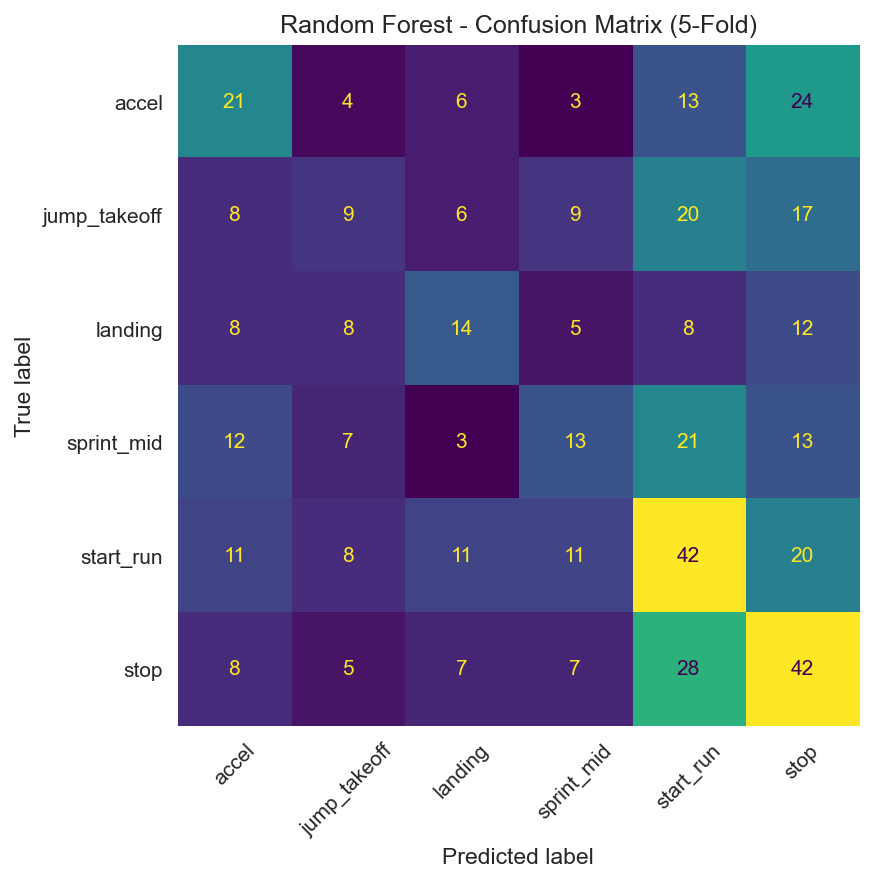
\includegraphics[width=0.8\linewidth]{images/confusion_matrix_5fold.png}
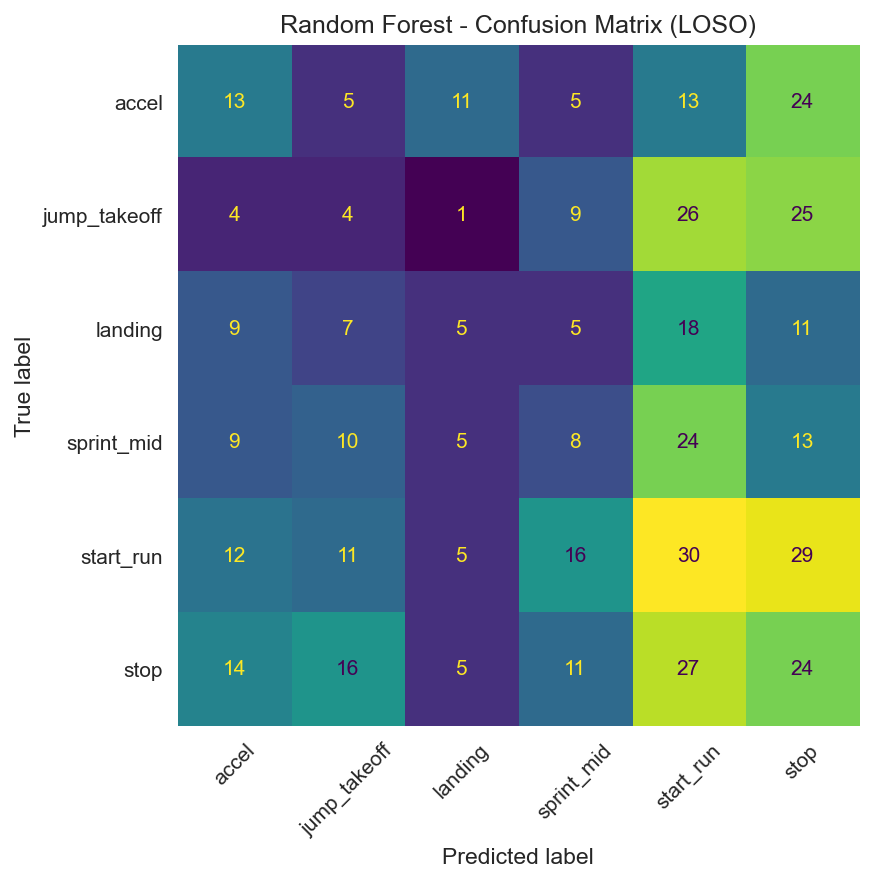
\includegraphics[width=0.8\linewidth]{images/confusion_matrix_loso.png}
\caption{Confusion matrices for the best-tuned Random Forest under 5-Fold CV (top) and LOSO CV (bottom).}
\label{fig:5FoldvsLOSOconfusion}
\end{figure}

\subsection{Error Analysis}
Error analysis focuses on LOSO results since 5-Fold CV can underestimate errors due to within-athlete data overlap across folds. Table~\ref{tab:misclassifications} lists the most frequent misclassification pairs under LOSO. The dominant error is \textit{Start\_Run} predicted as \textit{Stop} (34 times), which is notable because these two classes are temporal neighbours in the motion sequence; the sensor signal at the boundary between stopping and starting a run is ambiguous within a 1-second window.

\begin{table}[H]
\centering
\csvautotabular{csvFiles/topMisclassificationsLOSO.csv}
\caption{Most frequent misclassifications under LOSO evaluation.}
\label{tab:misclassifications}
\end{table}

\subsection{System Integration}
For full system integration, a prediction function was implemented so that new raw sensor recordings can be classified end-to-end without manual preprocessing. The function accepts a raw dataframe, applies the same windowing and z-score normalisation pipeline used during training, extracts the 20 consensus features, and passes the result to the saved best-model object for class prediction. This allows the pipeline to be reused on future athlete recordings without retraining. A known limitation is that the current integration was validated on the same cleaned dataset used for training rather than a truly independent recording, making it a consistency check rather than a deployment test.


\subsection{Overall Performance and Synthesis}
The best LOSO accuracy of 20.56\% (XGBoost) sits only marginally above the six-class random baseline of 16.7\%. All seven models exceed chance under 5-Fold CV, but LOSO performance confirms that learned representations do not transfer reliably to unseen athletes. This is consistent with a small dataset exhibiting high label noise from sliding-window assignment over rapidly-transitioning event labels.

\subsection{5-Fold vs LOSO Gap}
A consistent positive gap (5-Fold $>$ LOSO) is observed across all seven models. This gap has two sources:
\begin{enumerate}
    \item \textbf{Temporal leakage} from 50\% window overlap in 5-Fold splitting: adjacent windows from the same time segment can appear in both train and test folds, inflating 5-Fold estimates.
    \item \textbf{Athlete-specific signal characteristics} exploited when the same athlete appears in both train and test folds under 5-Fold CV.
\end{enumerate}
LOSO eliminates the second source, making it the appropriate metric for evaluating deployment readiness on unseen athletes.

\subsection{Feature Quality Limitations}
At approximately 10\,Hz with a 1.0\,s window, each window contains ten raw samples. Spectral features computed on ten points have a frequency resolution of 1\,Hz, barely sufficient to identify a dominant frequency below the Nyquist limit. This fundamentally constrains the information content of all spectral descriptors (dominant frequency, spectral energy, spectral entropy) in the current configuration, and may partly explain why gyroscope time-domain features ranked higher than spectral ones.

\subsection{Synthetic Data Caveat}
All numerical results must be interpreted in the context of a synthetically generated dataset. Real biosensor classification of motion phases typically achieves 70--90\% accuracy under comparable pipeline configurations~\cite{Vitali2020}. Near-chance performance here reflects the absence of class-discriminative signal structure in the synthetic generation process, not a failure of the pipeline design. The pipeline itself (preprocessing, sliding-window segmentation, feature extraction, and LOSO evaluation) follows established practice and would be directly applicable to real sensor data.

\section{Conclusion}
\label{sec:CONCLUSION}

\subsection{Summary of Findings}
This project designed and evaluated an end-to-end motion-phase classification pipeline for wearable biosensor data collected from five track-and-field athletes across six motion-phase classes.

The best LOSO accuracy of 20.56\% (XGBoost) sits only marginally above the six-class random baseline of 16.7\%. All seven models exceed chance under 5-Fold CV, but LOSO performance confirms that learned representations do not transfer reliably to unseen athletes. This is consistent with a small dataset exhibiting high label noise from sliding-window assignment over rapidly-transitioning event labels. A consistent positive gap (5-Fold $>$ LOSO) is observed across all models due to two sources: temporal leakage from 50\% window overlap in 5-Fold splitting, and athlete-specific signal characteristics exploited when the same athlete appears in both train and test folds. LOSO eliminates the second source, making it the appropriate metric for evaluating deployment readiness.

The full pipeline covered per-athlete z-score normalisation, sliding-window segmentation ($W=1.0$\,s, step 0.25), extraction of 69 features per window, and tuning of seven classifiers via \texttt{GridSearchCV}. Random Forest achieved the highest tuned 5-Fold CV accuracy (0.304), MLP the highest test accuracy (0.319), and XGBoost the best LOSO accuracy (0.206). A sweep of ten window sizes confirmed that 5-Fold accuracy rises with window size due to temporal leakage while LOSO remains near chance, confirming 5-Fold alone is an insufficient criterion for window-size selection.

\subsection{Limitations}
Results are constrained by several factors. First, the dataset is synthetically generated and does not replicate real biomechanical signal structure; real sensor classification typically achieves 70--90\% accuracy under comparable configurations~\cite{Vitali2020}, so near-chance performance here reflects absent class-discriminative signal rather than a pipeline failure. Second, with only five athletes, LOSO folds contain approximately 60 test windows each, making per-class metrics statistically unreliable. Third, at 10\,Hz with a 1.0\,s window, each window contains only ten raw samples; spectral features computed on ten points have a frequency resolution of 1\,Hz, barely sufficient to identify a dominant frequency below the Nyquist limit, which likely explains why gyroscope time-domain features ranked higher than spectral ones. Finally, no sensor-level signal filtering was applied, propagating high-frequency noise into all spectral features.

\subsection{Future Work}
Collecting real wearable sensor data with motion-capture ground truth would be the most impactful next step. Sensor-level low-pass filtering (e.g.\ Butterworth, 4\,Hz cutoff) on accelerometer and gyroscope channels should be evaluated before feature extraction. Retuning hyperparameters with LOSO as the inner-loop criterion would optimise models for cross-subject generalisation. Sequence-based architectures (LSTM, GRU, Conv1D) operating on the 3D reshaped tensors prepared in Section~\ref{sec:MODEL} are a natural extension, as they can exploit temporal dependencies across timesteps that hand-crafted features cannot capture.

\footnotesize
\bibliographystyle{IEEEtran}
\bibliography{bibliography}
\normalsize

\appendix

\section{Technical Notes}
\label{app:technical}

Key implementation details not covered in the main text are noted here. All code was written in Python 3 using scikit-learn~\cite{scikit-learn}, XGBoost~\cite{chen2016xgboost}, and Keras/TensorFlow. The notebook was executed in a single session; random seeds were fixed at \texttt{random\_state=42} throughout to ensure reproducibility. Feature extraction, model training, and evaluation are encapsulated in modular functions to allow re-execution on new data without modification of the pipeline logic.

\section{Member Contributions}
\label{app:contributions}

\begin{table}[H]
\centering
\small
\begin{tabularx}{\textwidth}{lp{3.2cm}X}
\toprule
\textbf{Member} & \textbf{Area} & \textbf{Tasks} \\
\midrule
\rowcolor{LightBlue} Sarah Loh       & Data Understanding \& Exploration  & Task 1: Dataset exploration: summary table, participant demographics, class distribution. Task 2: Annotated signal exploration, event plots, raw signal narrative. Task 9: Introduction \& Methodology sections. \\
Sneha Basnet    & Signal Processing \& Windowing     & Task 3: Signal preprocessing: filtering evaluation, interpolation, z-score normalisation, sensor range checks. Task 4: Windowing strategies, sliding window implementation, 10-size sweep, window selection justification. Task 9: Results \& Discussion section. \\
\rowcolor{LightBlue} Aye Nyein Kyaw  & Feature Engineering \& Analysis    & Task 5: Feature extraction: time-domain and frequency-domain features, importance visualisation, feature selection and interpretation. Task 9: Literature Review section. Task 8: Literature review group integration. \\
Nurislam Saliev & Modeling                           & Task 6: Classical models: Decision Tree, SVM, Naive Bayes, Random Forest, AdaBoost, XGBoost implementation and tuning. Deep learning extension, preprocessing pipeline, ANN sequence input preparation and architecture. Task 9: Results plots and model descriptions. \\
\rowcolor{LightBlue} Nathan Montero  & Evaluation \& Integration          & Task 7: Advanced evaluation: standard split (80/20), LOSO cross-validation, 10 window-size comparison with tables and plots, metrics table (precision, recall, accuracy, F1-macro), confusion matrices, error analysis. Final Discussion and Conclusion. \\
\bottomrule
\end{tabularx}
\caption{Team member task assignments and contributions.\label{tab:contributions}}
\end{table}


\end{document}